% Moise+ tutorial
%
% Jomi Fred H�bner


\documentclass[a4paper,pdftex,12pt]{report}


%
% Packages
% ========
%


\usepackage[latin1]{inputenc}
\usepackage[a4paper,pdftex,top=2cm,left=3.5cm,right=3.5cm,bottom=2cm]{geometry}

%\usepackage[brazil]{babel}
\usepackage{graphicx}                 % figuras
%\usepackage{floatflt}                % figuras como ``frames'' a direita
%\usepackage{wrapfig}                 % idem a floatflt, mas parece funcionar melhor 
\usepackage{subfigure}

\usepackage{latexsym}                 % mais s{\'\i}mbolos matem{\'a}ticos
\usepackage{amssymb}                  % mais s{\'\i}mbolos matem{\'a}ticos
%\usepackage{oz2e}                     % Z notation
\usepackage{theorem}

\usepackage{enumerate}                % permite apresentar um exemplo de como ser{\'a} a enumera{\c c}{\~a}o
\usepackage{tabularx}                 
\usepackage{booktabs}                 % melhora o desenho das tabelas com \toprule \midrule e \bottomrule
%\usepackage{showkeys}                % mostra os ref..... op{\c c}{\~o}es: [notref,notcite,final]

%\usepackage{makeidx}                  % {\'\i}ndice
%\makeindex
\usepackage{verbatim}


\RequirePackage[bf,center]{caption}
\RequirePackage{color}
\RequirePackage{url}
\RequirePackage{hyperref}        % PDF com links (pode-se usar como opção: dvipdfm, dvips, ...)
\hypersetup{colorlinks=true,urlcolor=blue,linkcolor=blue,citecolor=blue} % colorido
\RequirePackage{setspace}


\usepackage{algorithmic}
\usepackage[vlined, linesnumbered]{algorithm2e}

\newenvironment{remark}{\medskip\noindent \textsc{Remarks.}} {\medskip}


%\usepackage{listings}                 % for java listings
%\lstset{basicstyle=\footnotesize\sffamily,labelstep=1,labelstyle=\tiny,indent=1.2cm,extendedchars=true,frame=}
%\lstset{basicstyle=\footnotesize\sffamily,extendedchars=true,frame=}

\usepackage{xspace}

\usepackage{prettyref}                % facilita a constru{\c c}{\~a}o de refer{\^e}ncias, deve-se usar \prettyref{...}
\newrefformat{fig}{Figure~\ref{#1}}
\newrefformat{tab}{Table~\ref{#1}}
\newrefformat{sec}{Section~\ref{#1}}
\newrefformat{eq} {equation~(\ref{#1})}
\newrefformat{chp}{Chapter~\ref{#1}}
\newrefformat{ex} {example~\ref{#1}}
\newrefformat{ap} {appendix~\ref{#1}}
\newrefformat{alg}{algorithm~\ref{#1}}


%\usepackage{abnt-alf} % para as ref. no formato ABNT

\usepackage[sort]{natbib} % melhora as referencias (citep, citet, citeauthor, ...)
%\bibpunct{(}{)}{e}{a}{,}{,} 

\usepackage{acronym}

\sloppy

% Commands
% ========
%
\newcommand{\email}[2]{\href{mailto:#2}{#1}}
\renewcommand{\and}[0]{\\\vspace{6pt}}

\newcommand{\srctutorial}[0]{../../examples/tutorial}
\newcommand{\srcwritepaper}[0]{../../examples/writePaper}
\newcommand{\wpjason}[0]{jmoise/example/writePaper}

\newcommand{\toindex}[1]{\index{#1}\marginpar{\scriptsize{\textsf{i:#1}}}}
\newcommand{\indexdef}[1]{\index{#1|textsl}\marginpar{\scriptsize{\textsf{id:#1}}}}

\newcommand{\defEventoOrg}[5]{
  \vspace{.5cm}
  \noindent
  \begin{tabular}{l l}
    \toprule
    Evento         & #1 \\
    \midrule
    Argumentos     & #2 \\
    \midrule
    Pr{\'e}-condi{\c c}{\~o}es  & #3 \\
    \midrule
    Efeitos        & #4 \\
    \bottomrule
  \end{tabular}
  \vspace{.5cm}

  \noindent #5
}


\newcommand{\tdef}[0]{\; =_{\textrm{\tiny{def}}} \;} %stackrel{\triangle}{=}
\newcommand{\tq}[0]{\;\;\textrm{tal que}\;\;}
\newcommand{\subrole}[0]{\sqsubset}

\newcommand{\ie}[0]{isto {\'e}}
\newcommand{\eg}[0]{por exemplo}

\theorembodyfont{\rmfamily}
\newtheorem{tdefn}{Defini{\c c}{\~a}o}[chapter]
\newtheorem{texplo}{Exemplo}[chapter]
  
\newenvironment{defn}[1]
   {\begin{tdefn}\label{def:#1}}
   {\hfill$\Box$\end{tdefn}}
\newenvironment{definicao}[2]
   {\begin{tdefn}\label{def:#2}\textbf{(\textsl{#1})}}
   {\hfill$\Box$\end{tdefn}}
\newenvironment{explo}
   {\begin{texplo}}
   {\hfill$\Box$\end{texplo}}


\newcommand{\pendencia}[1]{~[\textsc{Pend{\^e}ncia}\footnote{\textbf{#1}}]~}
%\newcommand{\pendencia}[1]{}

\newcommand{\processo}[1]{\textsc{#1}}
\newcommand{\RETURN}[0]{\textbf{return}\xspace}
\newcommand{\evento}[1]{\textsl{#1}}
\newcommand{\papel}[1]{\textsl{#1}}
\newcommand{\relacao}[1]{\textsf{#1}}
%\newcommand{\pode}[2]{#1 \relacao{pode} #2}
%\newcommand{\deve}[2]{#1 \relacao{deve} #2}
\newcommand{\pode}[0]{permission}
\newcommand{\deve}[0]{obligation}
\newcommand{\compat}[0]{\bowtie}

%\newcommand{\compat}[2]{#1 \relacao{compat} #2}

\newcommand{\group}[1]{\texttt{#1}}
\newcommand{\role}[1]{\textsf{#1}}
\newcommand{\agent}[1]{$#1$}
\newcommand{\goal}[1]{\textsl{#1}}

\newcommand{\igroup}[0]{grupo\xspace}
\newcommand{\igroups}[0]{grupos\xspace}
\newcommand{\tgroup}[0]{especifica{\c c}{\~a}o de grupo\xspace}
\newcommand{\tgroups}[0]{especifica{\c c}{\~a}o de grupos\xspace}


\newcommand{\Taems}[0]{{\sc T{\ae}ms}\xspace}
\newcommand{\taems}[0]{{\sc t{\ae}ms}\xspace}
\newcommand{\aalaadin}[0]{{\sc Aalaadin}\xspace}
%\newcommand{\Moise}[0]{{\sc Moise}\xspace}
%\newcommand{\moise}[0]{{\sc moise}\xspace}

% o \textsc n{\~a}o funcina dentro de t{\'\i}tulos
\newcommand{\moise}[0]{$\mathcal{M}${\sc{oise}}\xspace}
\newcommand{\moisem}[0]{$\mathcal{M}${\sc{oise}}$^{+}$\xspace}
\newcommand{\smoisem}{\mbox{$\mathcal{S}$-\moisem}\xspace}
\newcommand{\jmoisem}{\mbox{$\mathcal{J}$-\moisem}\xspace}
\newcommand{\saci}[0]{\textsc{Saci}\xspace}
\newcommand{\Jason}{\textit{\textbf{Jason}}\xspace}
\hyphenation{Jason}



% \renewcommand{\maketitle}{
%   \newpage
%   \thispagestyle{empty}
%   \null
%   \begin{center}


%     \begin{spacing}{2}
%       \vspace{\stretch{1}}
%       \textbf{\huge \@title}
%     \end{spacing}
%     \vspace{1cm}
    
%     \@author
%     \vspace{24pt}
    
%     %\@institution

%     \vspace{\stretch{2}}
%     %\@place \\ 
%     \@date

%   \end{center}

%   \hypersetup{pdftitle=\@title,pdfauthor=\@author}
% }


\begin{document}


\title{\moise tutorial \\ {\footnotesize (for \moise 0.7)}}

\author{
    \email{Jomi Fred H�bner}{jomi@das.ufsc.br}$^{1}$\\
    \email{Jaime Sim�o Sichman}{jaime.sichman@poli.usp.br}$^{2}$\\
    \email{Olivier Boissier}{Olivier.Boissier@emse.fr}$^{3}$\\[.5cm]
    %
    $^1$ \small{\href{http://www.das.ufsc.br}{Universidade Federal de Santa Catarina}}\\
    $^2$ \small{\href{http://www.usp.br}{Universidade de S�o Paulo}}\\
    $^3$ \small{\href{http://www.emse.fr}{�cole Nationale Sup�rieure des Mines de Saint-�tienne}}\\
}

\date{\small{2010}}


\maketitle


\tableofcontents
%\listoffigures
%\listoftables

% Acronimos
\chapter*{Acronyms}
%\addcontentsline{toc}{chapter}{Lista de Abreviaturas}
\begin{acronym}
\acro{NS}{Normative Specification}
\acro{FS}{Functional Specification}
\acro{MAS}{Multi-Agent System}
\acro{MOISE}{Model of Organisation for multI-agent SystEms}
\acro{OS}{Organisational Specification}
\acro{OE}{Organisational Entity}
\acro{SCH}{Social Scheme}
\acro{SS}{Structural Specification}
\end{acronym}


\chapter{Introduction}

This tutorial describes how to \emph{specify} and \emph{program} a
\ac{MAS} organisation using the \moise model. Moreover, this tutorial
focus on the utilisation of the \moise computational tools. It is
assumed that the reader knows the \moise purpose and fundamental
concepts (presented in \cite{hubner:02b,hubner:07,hubner:09c}, which
can be found in the publications directory of \moise distribution). A
complete list of related publications is available at
\url{http://moise.sourceforge.net/related-papers.html} and more
detailed documentation is also available with the distribution in the
directory \texttt{doc}.


% Since the implementation of these computational tools gets into
% details of model\ldots some of this operational details are described here.

\section{A general view of the soccer example}

Throughout the text, a soccer team is used as an example. A soccer
team that we will specify is formed by players with roles like
goalkeeper, back player, leader, attacker, coach, etc. These role
players are distributed in two groups (defense and attack) which form
the main group (the team group). The team structure is specified,
using the \moise notation, in the \prettyref{fig:jojTeam} (the next
chapter will explain the details of the notation and its
interpretation).

\begin{figure}
  \begin{center}
    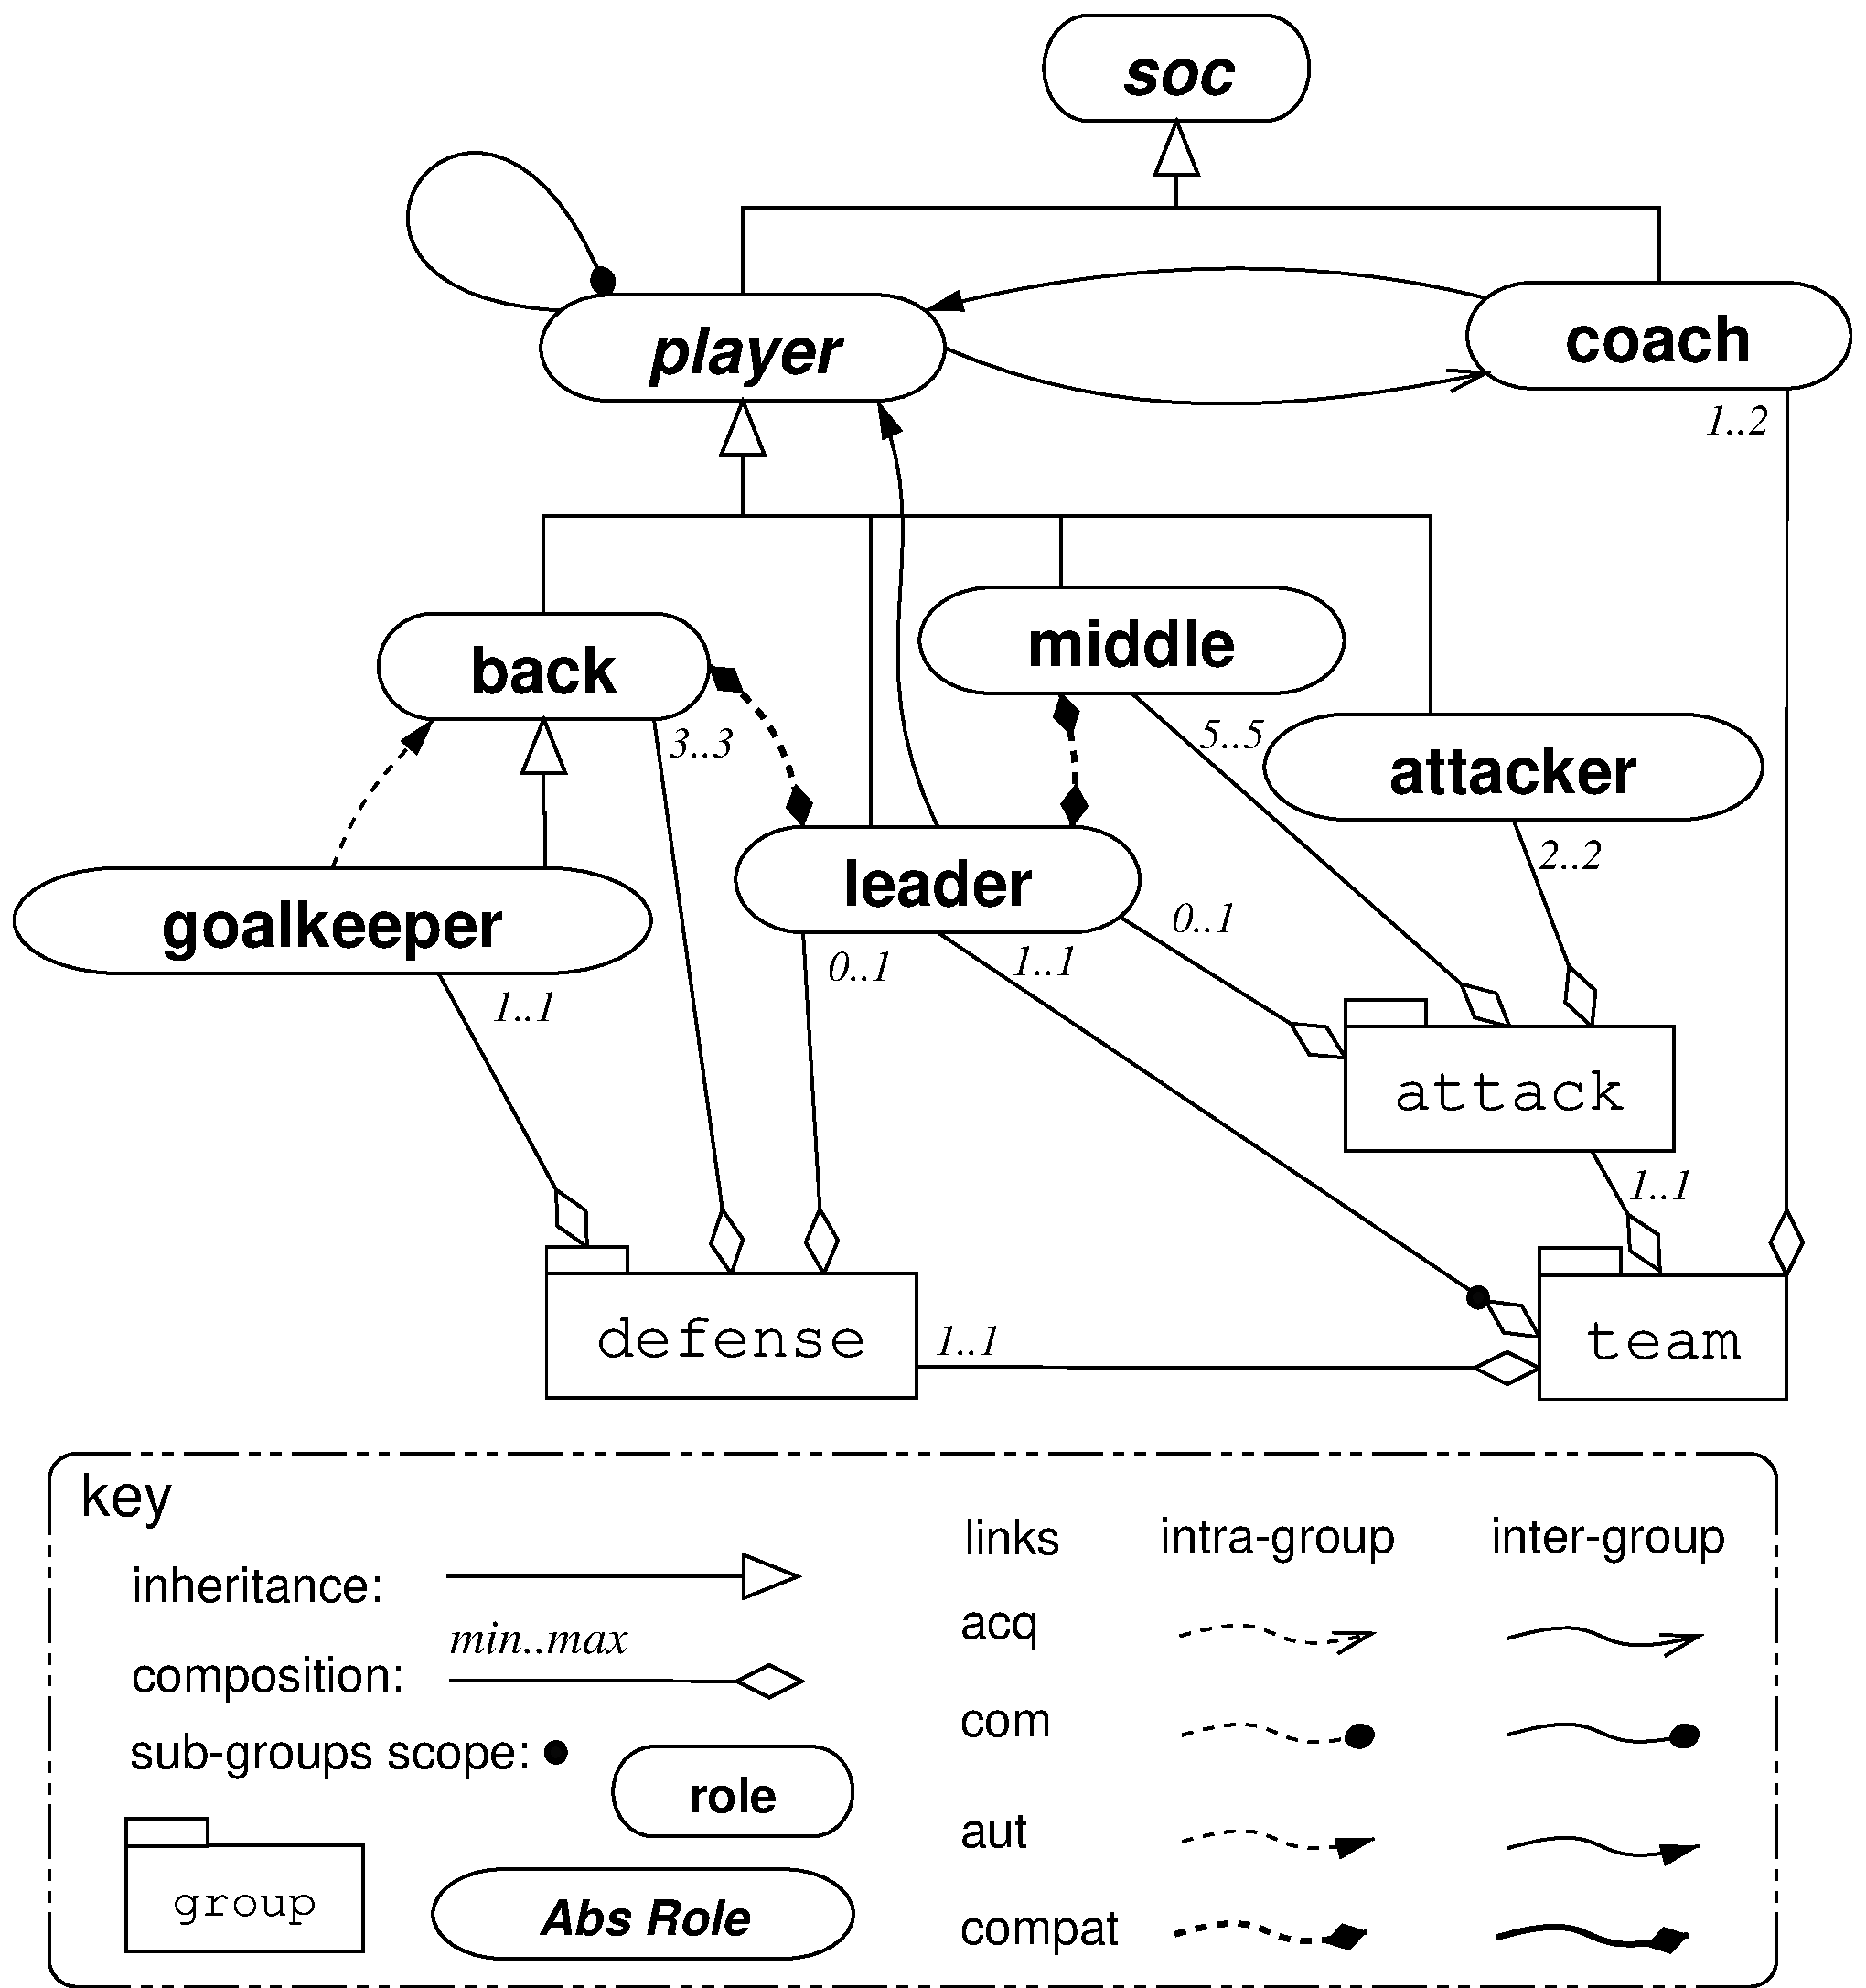
\includegraphics[width=.7\textwidth]{\srctutorial/figures/jojTeam4-en.pdf}
  \end{center}
  \caption{The structure of the soccer team}
  \label{fig:jojTeam}
\end{figure}

The team also has some rehearsed plays, one of them is specified by
the \ac{SCH} depicted in the \prettyref{fig:jojSCH}. This scheme has
three missions ($m_1$, $m_2$, and $m_3$) and their respective goals
(the mission $m_3$ has, for example, the goals `be placed in the
opponent goal area', `shot at the opponent's goal', and, a common
goal, `score a goal'). Agents playing these roles may commit to
this scheme missions according to \prettyref{tab:jojDS}.


\begin{figure}
  \begin{center}
    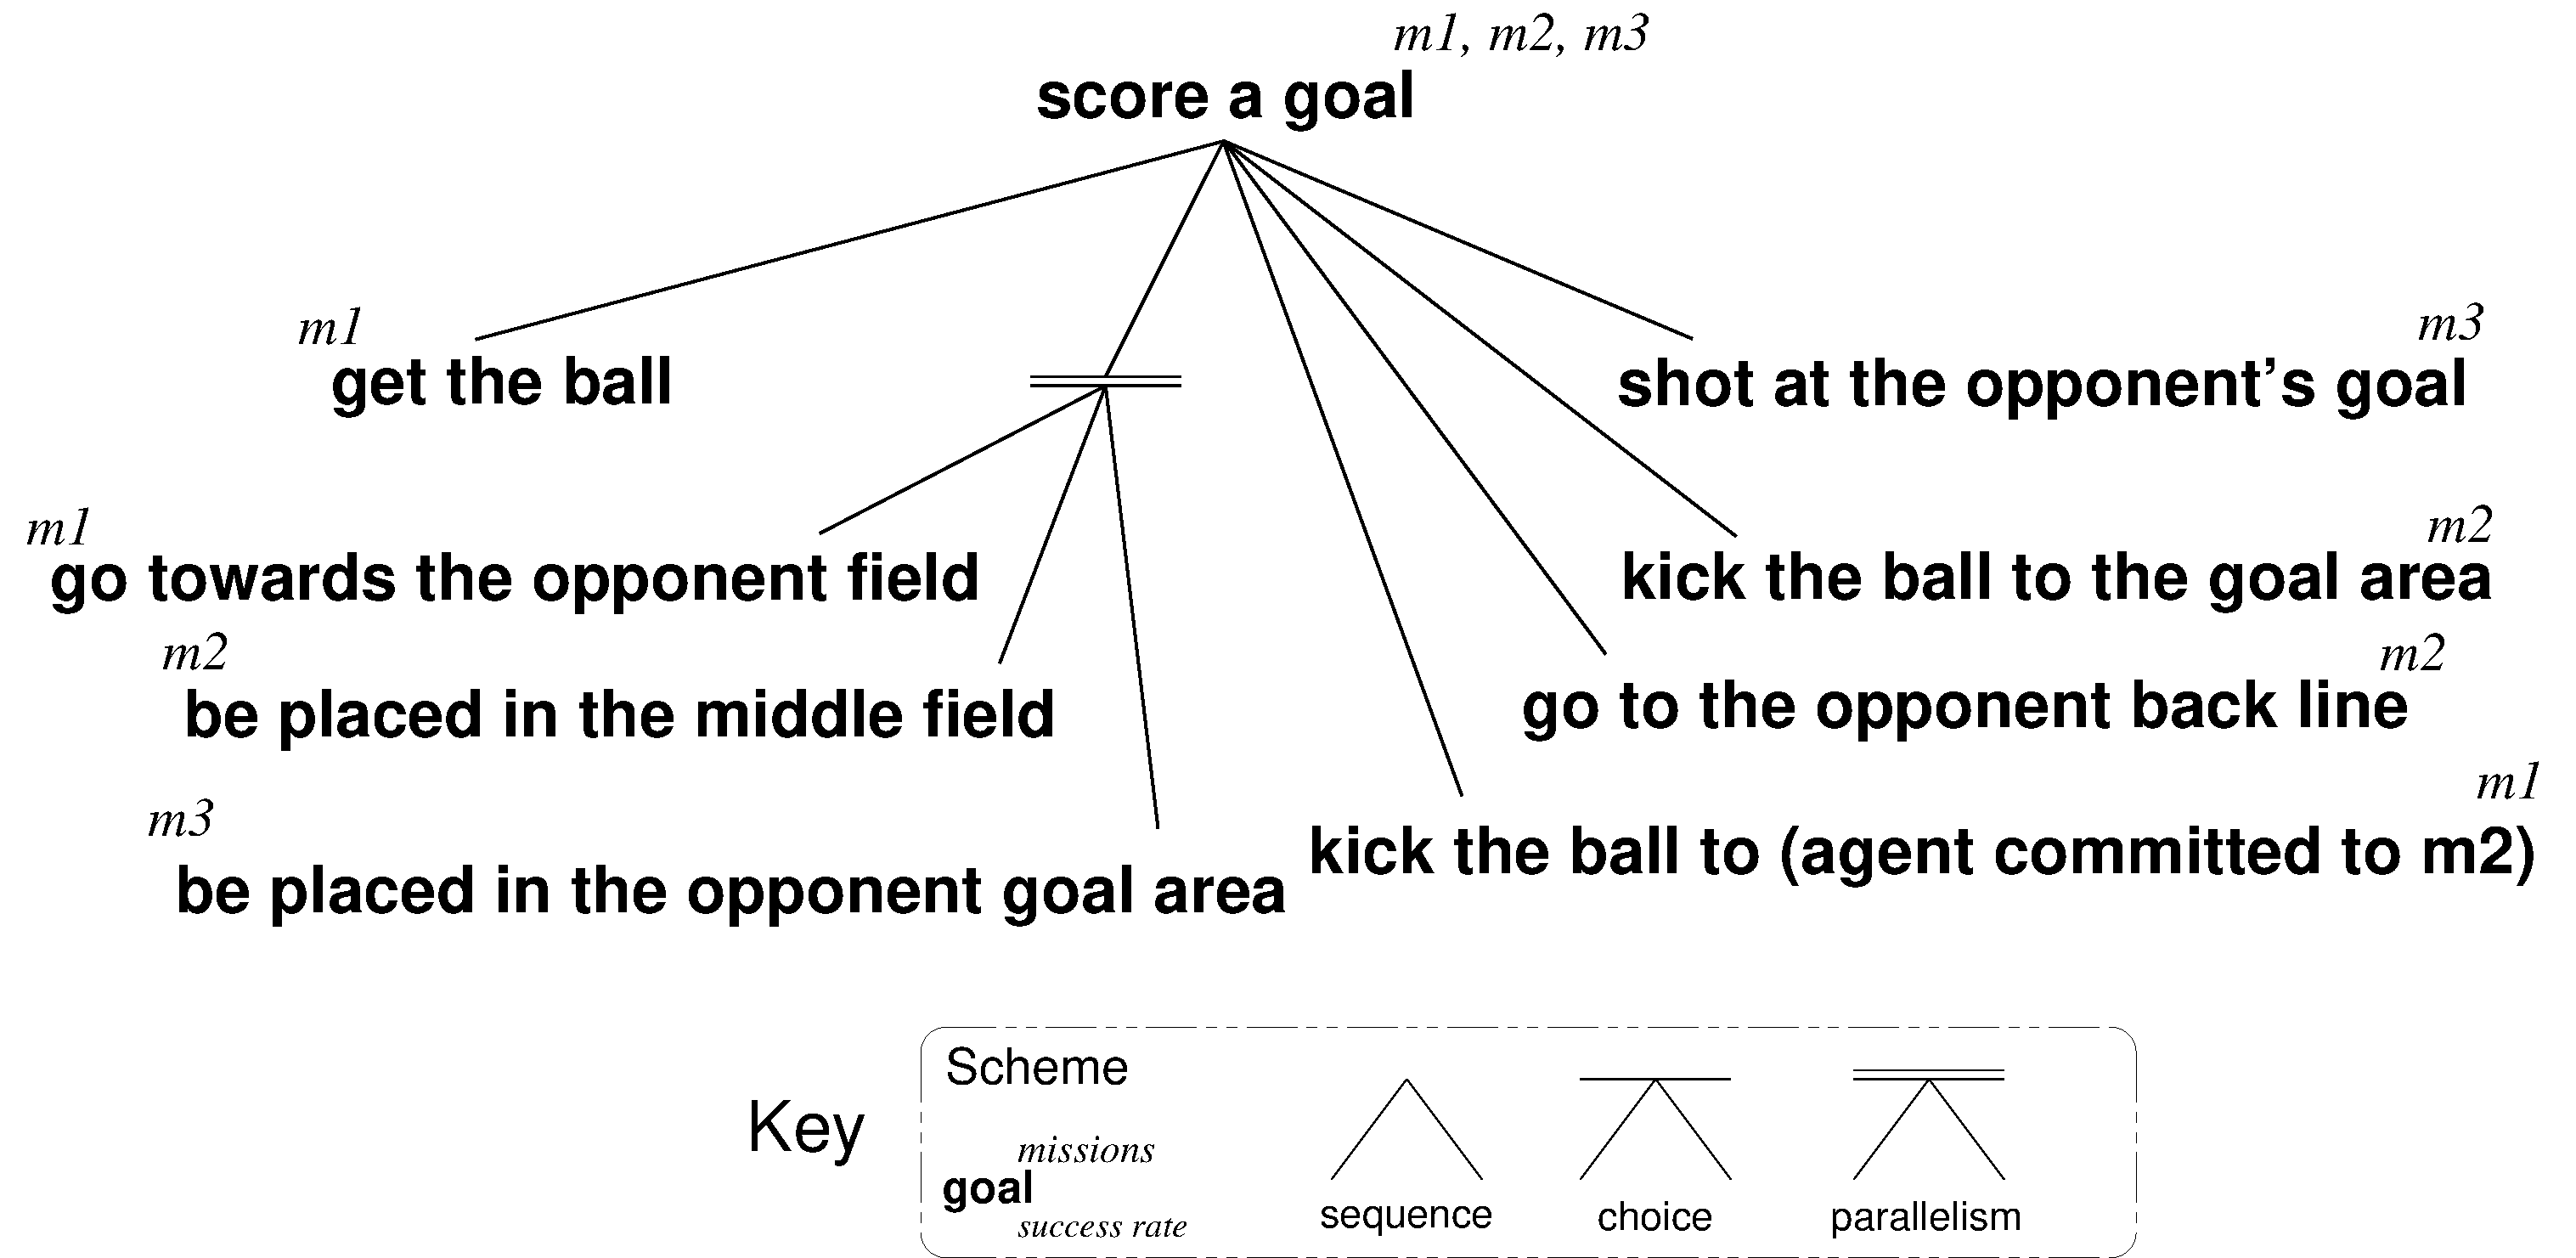
\includegraphics[width=\textwidth]{\srctutorial/figures/jojSCH2-en.pdf}
  \end{center}
  \caption{A scheme of the soccer team}
  \label{fig:jojSCH}
\end{figure}


\begin{table}
  \begin{center}
    \begin{tabular}{c c c c c}
      \toprule
      role & deontic relation & mission\\
      \midrule
      back     & $\pode$ & $m_1$\\
      middle   & $\deve$ & $m_2$\\
      attacker & $\deve$ & $m_3$\\
      \bottomrule
    \end{tabular}
    \caption{Normative Specification}
    \label{tab:jojDS}
  \end{center}
\end{table}

The structural, functional, and deontic specifications briefly
described above form the \ac{OS} of a soccer team that, for example,
11 players can `instantiated' building the \ac{OE} of
\prettyref{tab:oeAgents}.

\begin{table}
\begin{center}
  \begin{tabular}{l l l}
    \toprule
    agent & role & in group\\
    \midrule
    Marcos     & goal-keeper & defense \\
    Lucio      & back & defense \\
    Edmilson   & back & defense\\
    Roque Jr.  & back & defense \\
    Cafu       & leader and middle & attack\\
    Gilberto Silva & middle & attack \\
    Juninho    & middle & attack\\
    Ronaldinho & middle & attack\\
    Roberto Carlos & middle & attack\\
    Ronaldo    & attacker & attack\\
    Rivaldo    & attacker & attack\\
    Scolari    & coach & team\\
    \bottomrule
  \end{tabular}
  \caption{Organisational Entity}
  \label{tab:oeAgents}
\end{center}
\end{table}


\section{The writing paper example}\label{sec:exeWP}

Another example used in this document is the `writing paper',
initially described in \cite{kitio:07} and then extended in
\cite{hubner:09e}. In this second example, we consider a set of agents
that wants to write a paper and therefore define an organisational
specification to help them.  This MAS structure has one group
(\group{wpgroup}) with two roles, editor and writer, both are sub-role
of the author role. The links and cardinalities of this group are
specified, using the \moise notation, in the \prettyref{fig:wpSS}. A
complete description in XML can be found in the \prettyref{ap:wp}.

\begin{figure}
  \begin{center}
    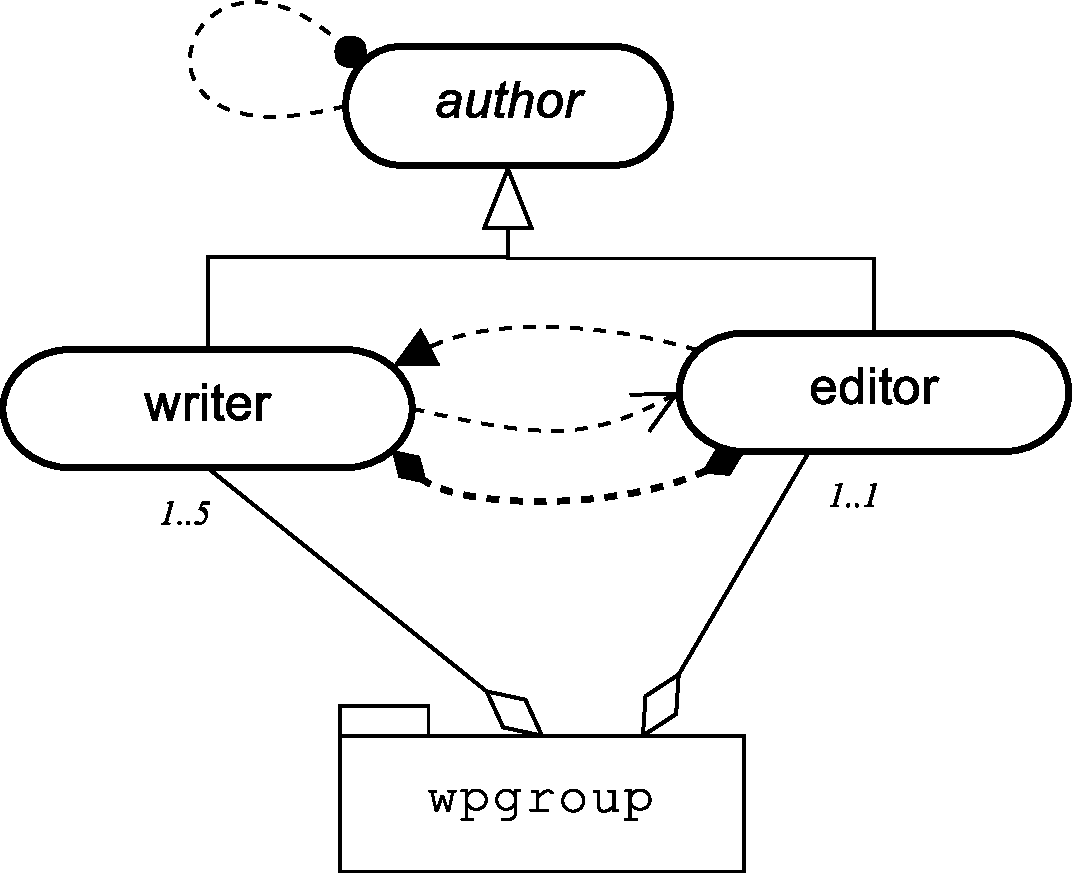
\includegraphics[width=.5\textwidth]{\srcwritepaper/figures/writePaperSS.pdf}
  \end{center}
  \caption{The write paper structure}
  \label{fig:wpSS}
\end{figure}
To write a paper, they developed a scheme where initially the editor
defines a draft version with title, abstract, introduction, and
section names, this step is represented by the goal \goal{fdv}. Then
the writers `fill' the gaps of the paper's sections to get a
submission version of the paper, represented by the global goal
identified by \goal{sv}. This scheme is detailed in
\prettyref{fig:wpFS}, note that the goals \goal{wcon} (write the
conclusion) and \goal{wref} (build the references) can be performed in
parallel. There is a mission for the editor ($mMan$), a mission for
the writers ($mCol$), and another mission for writers ($mBib$ --- get
the references for the paper). This relation from roles to missions is
specified in \prettyref{tab:wpDS}.  Note that some goals have not a
mission assigned, in this case, the achievement of the goal depends on
the achievement of the sub-goals. For instance, the goal \goal{sv} is
achieved with the goals \goal{wsec} and \goal{finish} are achieved.



\begin{figure}
  \begin{center}
    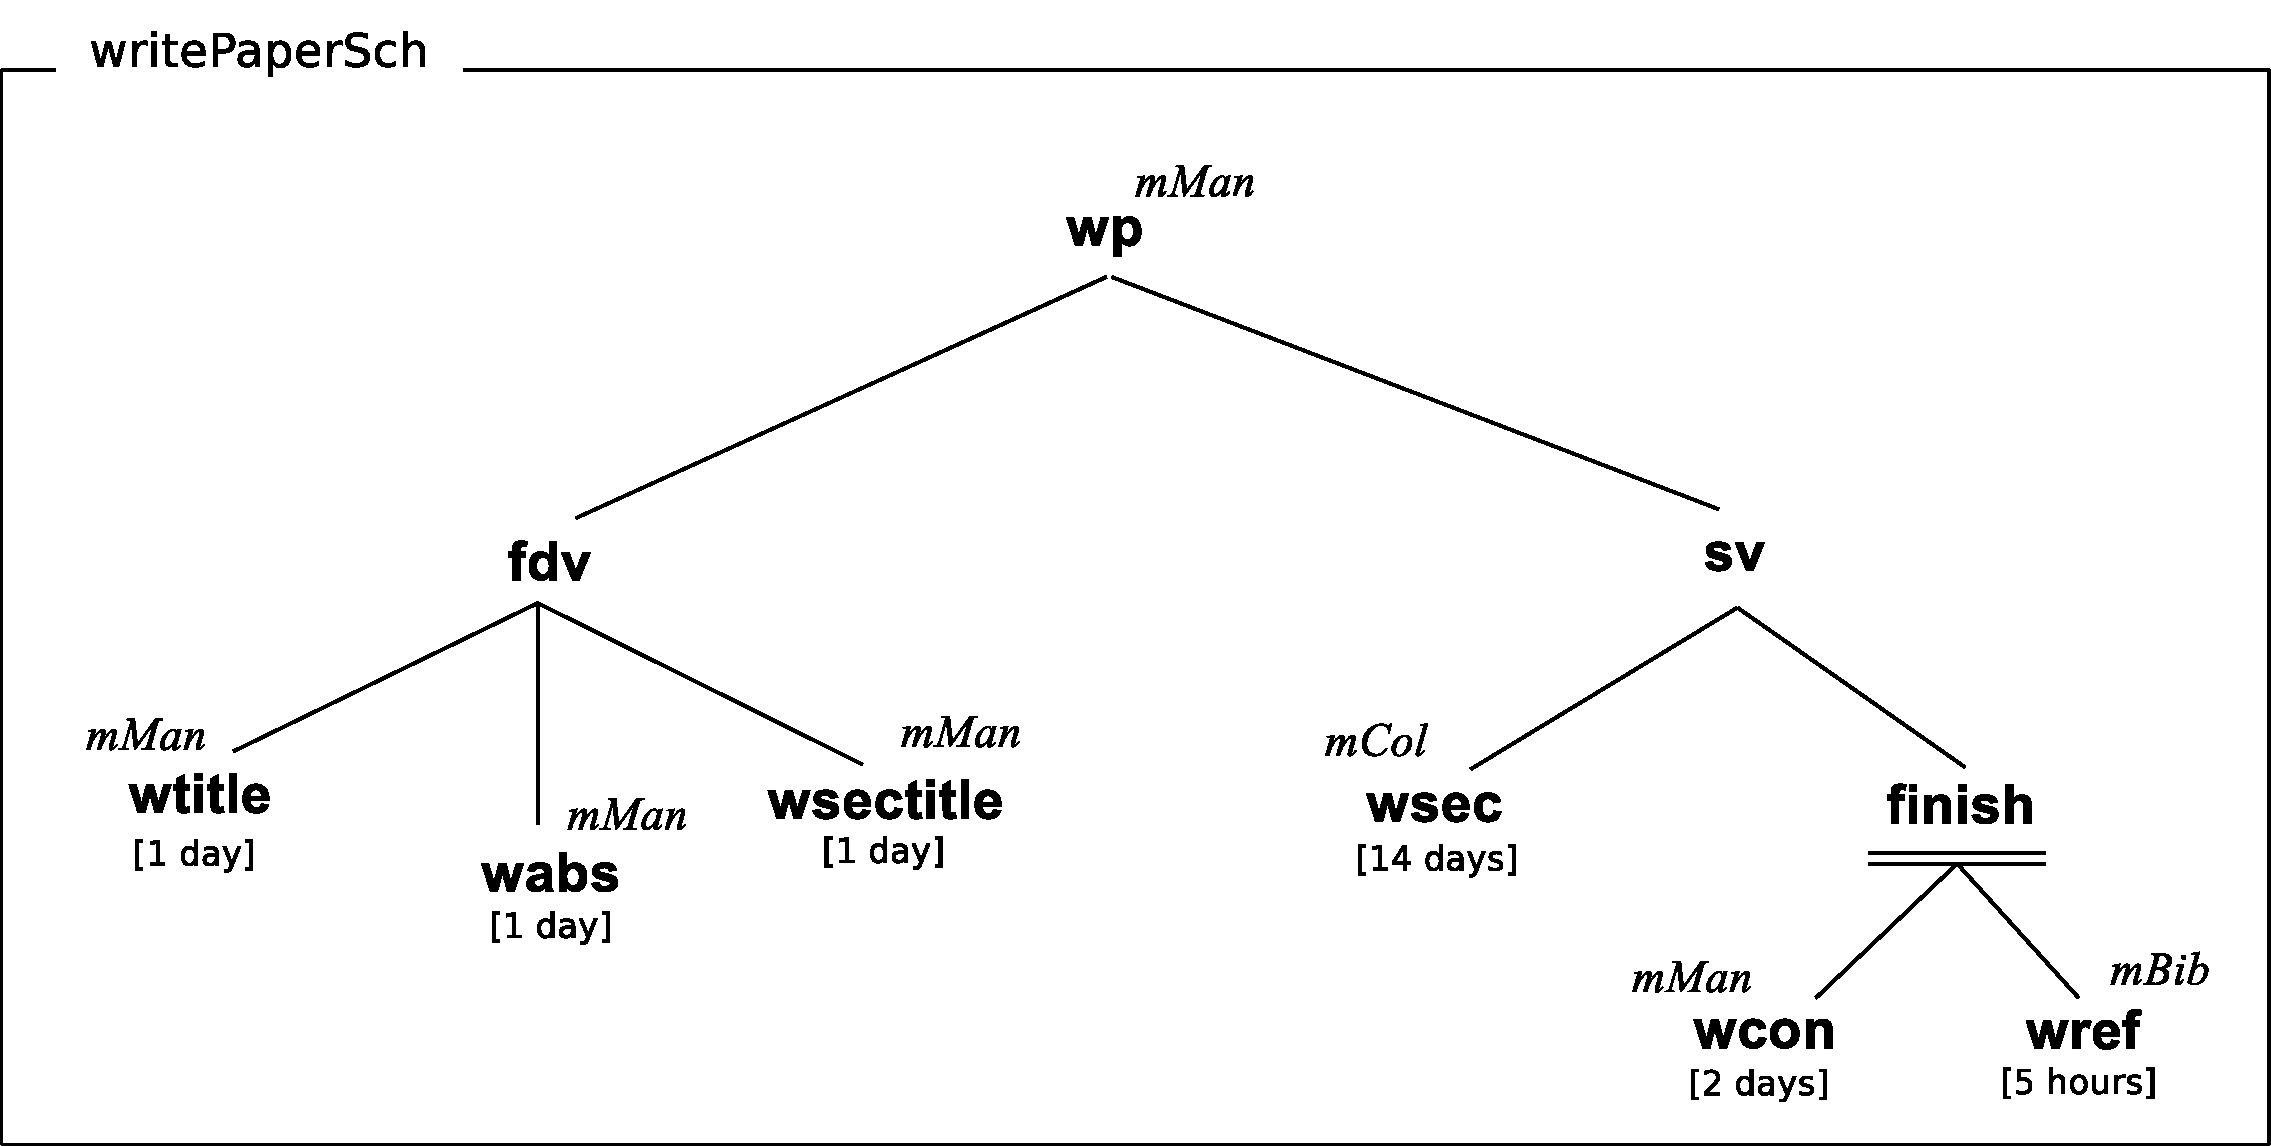
\includegraphics[width=.9\textwidth]{\srcwritepaper/figures/writePaperFS.pdf}
    \begin{tabular}{c c c c}
      \toprule
      mission & cardinality \\
      \midrule
      $mMan$ & 1..1 \\
      $mCol$ & 1..5 \\
      $mBib$ & 1..1 \\
      \bottomrule
    \end{tabular}
  \end{center}
  \caption{The write paper scheme}\label{fig:wpFS}
\end{figure}


\begin{table}
  \begin{center}
    \begin{tabular}{c c c c c}
      \toprule
      role & deontic relation & mission & TTF\\
      \midrule
      editor  & $\pode$ & $mMan$ \\
      writer  & $\deve$ & $mCol$ & 1 day \\
      writer  & $\deve$ & $mBib$ & 1 day\\
      \bottomrule
    \end{tabular}
    \caption{Normative Specification}
    \label{tab:wpDS}
  \end{center}
\end{table}

The structural, functional, and deontic specifications briefly described above
form an \ac{OS} that, for example, 3 agents can `instantiated' building the
\ac{OE} of \prettyref{tab:oeAgentsWP}.

\begin{table}
\begin{center}
  \begin{tabular}{l l l l}
    \toprule
    agent & role & in group & mission \\
    \midrule
    Jaime     & editor & wpgroup & $mMan$\\
    Jomi      & writer & wpgroup & $mCol$ \\
    Olivier   & writer & wpgroup & $mCol$ \\
    Olivier   & writer & wpgroup & $mBib$ \\
    \bottomrule
  \end{tabular}
  \caption{Write paper Organisational Entity}
  \label{tab:oeAgentsWP}
\end{center}
\end{table}



\section{Structure of the remaining text}

The creation of the soccer team entity is initially done in a \moise
OE dynamics simulator (described in \prettyref{chp:simulator}). The
objective of this simulator is to allow the designer to test the
organisational specification by performing actions like agent entrance,
role adoption, scheme creation, group creation, etc. No knowledge
about any programming language is required to use this simulator, it
focus only on the organisational specification and simulation.

To program the agents, appendixes \ref{chp:jmoisem} and
\ref{chp:smoise} present two tools where agents can be programmed
using \moise concepts. While in the latter tool, the agents are
programmed in Java, in the former, the AgentSpeak language is
used. Note however that these tools are \emph{outdated}, we are
currently using a new platform based on artifacts, called ORA4MAS
\cite{hubner:09c}. The documentation related to this platform is
available in the \moise distribution in the directory
\texttt{doc/ora4mas}.


%
%  Simulator
%  ---------
%
\chapter{Organisational Entity Dynamics Simulator} 
\label{chp:simulator}

This chapter explains both how to write an \ac{OS} for the \moise
tools and how to use the simulator to test this OS.

% --------------------
\section{Installation}

In order to start using the \moise tools  you need to perform to
following steps:
\begin{enumerate}
  
\item check whether the Java 1.5 is installed in your system (the
  \texttt{java} command must be in the PATH);

\item download the \moise platform from
  \url{http://moise.sourceforge.net} and \Jason programming language from
  \url{http://jason.sourceforge.net}.

\item uncompress the downloaded files; and
  
\item test the system by running the script \texttt{\ldots/bin/simOE}
  (or \texttt{ant run}).  The simulator asks for a specification file,
  select the \texttt{example/tutorial/jojOS.xml} and a screen like
  \prettyref{fig:fsc} should appear.

  \begin{figure}
    \begin{center}
      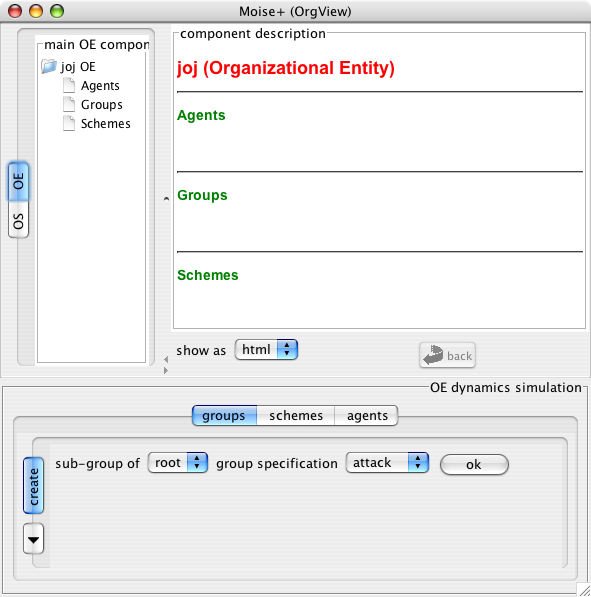
\includegraphics[width=.8\textwidth]{screens/firstScreen.png}
    \end{center}
    \caption{Simulator first screen}
    \label{fig:fsc}
  \end{figure}

\end{enumerate}


% --------------------
\section{Structural Specification} \label{sec:ss}

The first step to build the \ac{SS} of the soccer team
(\prettyref{fig:jojTeam}) is to write a XML file that describes its
structure.\footnote{The XML files have to follow the XML Schema
  \texttt{src/xml/os.xsd}.} The next sections present how this file is
composed (all the content of this file is listed in
\prettyref{ap:joj}). The focus is both on the XML tags and on some
implementation issues.


\subsection{Role definition (individual level)}

The following lines define the role inheritance relation:
\begin{verbatim}
<role-definitions>
  <role id="player" />
  <role id="coach" />
  <role id="middle"> <extends role="player"/> </role>
  <role id="leader"> <extends role="player"/> </role>
  ...
</role-definitions>
\end{verbatim}

\vspace{.5cm}

\begin{remark}
\begin{itemize}
  
\item The role \role{soc} is the root of the role inheritance tree.
  All roles are sub-roles of \role{soc}, even if it is not explicitly
  specified, as is the case of role coach.
  
\item A role definition does not imply that an agent is allowed to
  play it, only when the role is added in a group specification it can
  be played. The roles definition tag is used simply to state the
  roles hierarchy.
  
\item To state that a role inherits properties from many other roles,
  the \texttt{extends} tag can be used many times, for example:
  \begin{verbatim}
    <role id="r1> 
      <extends role="r2" />
      <extends role="r3" />
    </role>
  \end{verbatim}
\end{itemize}
\end{remark}


% \subsection{Link types definition (social level)}

% The following lines define the possible types for links between roles:
% \begin{verbatim}
% <link-types>
%   <link-type id="authority"/>
%   <link-type id="acquaintance"/>
%   <link-type id="communication"/>
% </link-types>
% \end{verbatim}
% Although the \moisem proposes these three link types, some application
% domains may extend this set adding a new \textsf{link-type} tags.


\subsection{Groups definition (collective level)}

A group specification is described inside the tag
\texttt{group-specification}, for example:
\begin{verbatim}
<group-specification id="team">
    ...
</group-specification>
\end{verbatim}
creates the group specification identified by \group{team}. Inside the
group specification, we can include:

\begin{itemize}

\item the allowed \emph{roles} in this group and their cardinality. For
  example, the following XML code states that one or two agents can
  play the role \role{coach} in the group \group{team}:
  \begin{verbatim}
    <roles>
        <role id="coach" min="1" max="2"/>
    </roles>
  \end{verbatim}

  The cardinality is optional, the default value for min is 0 and for max
  is `unlimited'.

  All roles included inside a group must be previously defined inside
  the \texttt{role-definitions} tag.
  
\item the \emph{links} between the group's roles, for example, to
  state an inter-group authority link from \role{coach} to
  \role{player}:
  \begin{verbatim}
    <link from="coach"  
          to="player" 
          type="authority"     
          scope="inter-group" 
          extends-subgroups="true" />
  \end{verbatim}
  
  The values for the link \texttt{type} are `authority',
  `communication', and `acquaintance'.
  
  The values for the \texttt{scope} are `inter-group' and
  `intra-group'.

  In case where \texttt{extends-subgroups} parameter is \emph{true},
  this link is also valid in all \group{team} subgroups. The
  default value is \emph{false}.

\item the \emph{subgroups} and their cardinality:
  \begin{verbatim}
    <subgroups>
      <group-specification id="attack" min="1" max="1">
        ...
      </group-specification>
                
      <group-specification id="defense" min="1" max="1">
        ...
      </group-specification>
    </subgroups>
  \end{verbatim}
  Each subgroups also contains a group specification.
  
\item the \emph{constraints} formation. For example, in the group
  \group{attack} there are the following role compatibility:
  {\small
  \begin{verbatim}
    <formation-constraints>
      <compatibility from="middle" 
                     to="leader"
                     scope="intra-group" 
                     extends-subgroups="false" 
                     bi-dir="true"/>
    </formation-constraints>
  \end{verbatim}
  }
  If the \texttt{bi-dir} parameter is \emph{true}, the compatibility
  (or link) also exists from the destination to source.

\end{itemize}


\subsection{Organisational Entity creation}

Given the XML file described in the previous sections, we can create
organisational entities, groups, agents, etc.  Notice however that
only the structure is specified yet.

To create an \ac{OE}:
\begin{enumerate}

\item Run the \texttt{\ldots/bin/simOE} script.
  
\item Open the soccer team \ac{SS} file
  (\ldots/examples/tutorial/jojSS.xml).

\item A screen like \prettyref{fig:fsc} appears: an OE with an OS but
  without groups, agents, or schemes.

\item You can navigate through the OS specification clicking on the `OS'
  tab and after in the `joj' tree object (\prettyref{fig:os1}).

  \begin{figure}
    \begin{center}
      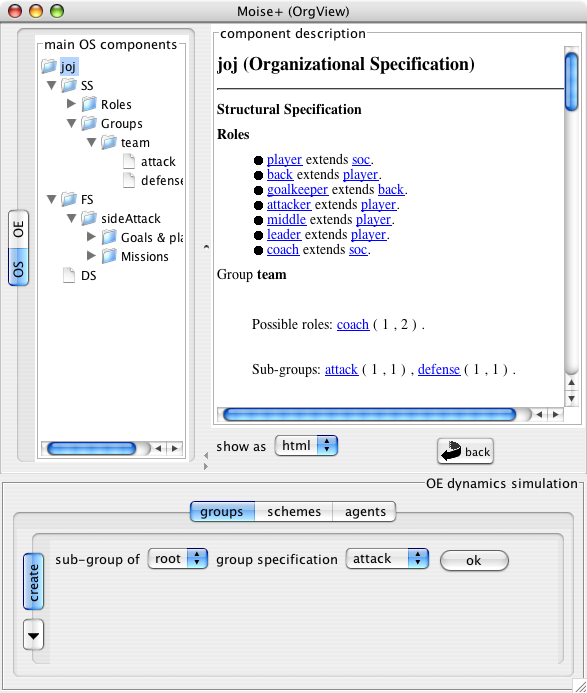
\includegraphics[width=\textwidth]{screens/os1.png}
    \end{center}
    \caption{Organisational Specification}
    \label{fig:os1}
  \end{figure}
\end{enumerate}



\subsection{Group creation}


\begin{enumerate}
  
\item To create a group, select the `group'/`create' tab, then select
  the creation of a `root' group (some group that is not subgroup
  of any other group), select the `team' specification, and finally 
  click on `ok' button.
  
  Notice that a new group (id=gr\_team0)\footnote{The id of the group is
    automatically given by the simulator. In the API however, the id of the
    group may be defined when it is created.} was created and its well
  formation status is not Ok (\prettyref{fig:gr1}).
  \begin{figure}
    \begin{center}
      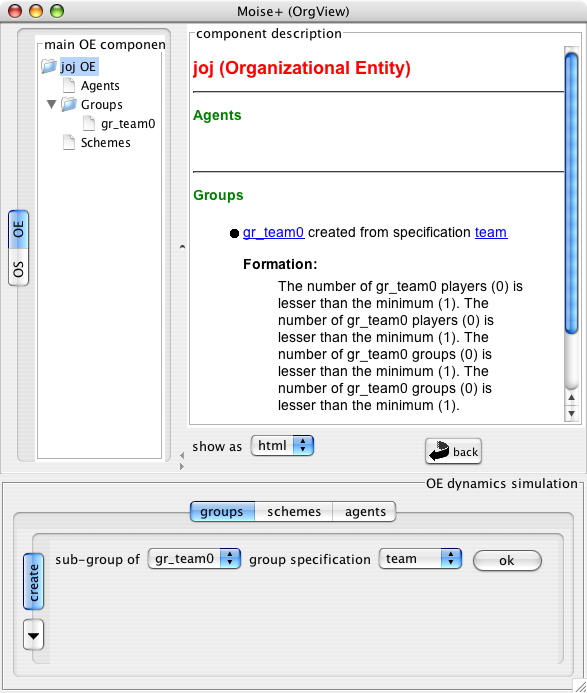
\includegraphics[width=\textwidth]{screens/gr1.png}
    \end{center}
    \caption{Result of the first group creation}
    \label{fig:gr1}
  \end{figure}
  
\item Create a \group{gr\_team0} subgroup using the defense
  specification. Notice that a defense group can only be created as a
  \group{team} subgroup, since defense is specified as a \group{team}
  subgroup in the SS.
  
\item Create another \group{gr\_team0} subgroup using the attack
  specification.

\end{enumerate}



\subsection{Agent creation}

To create an agent, select the `agent'/`create' tab, fill
`Marcos' in the agent name field, and click on `create' button.
Do the same for the other agents enumerated at page
\pageref{tab:oeAgents}. %The agent creation event has no constraints.


\subsection{Role adoption}

To assign roles to agents, as suggested in \prettyref{tab:oeAgents},
select the `agent'/`roles' tab, select the agent (e.g. Marcos),
select the role (e.g. `goalkeeper'), select the group
`gr\_defense1', and click on the `ok' button (see
\prettyref{fig:role1}). Repeat this operation for the other players'
roles and notice how the groups' well formation status is changing.

\begin{figure}
  \begin{center}
    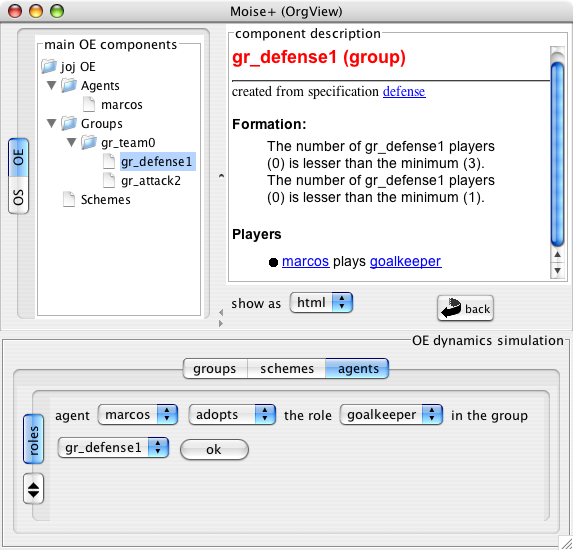
\includegraphics[width=.8\textwidth]{screens/role1.png}
  \end{center}
  \caption{Role adoption result}
  \label{fig:role1}
\end{figure}

The role adoption event is constrained by the cardinality and
compatibilities of each role. For example, try the following role
adoption and notice the error messages:

\begin{itemize}
\item Marcos adopts the role \role{back} in the group \group{gr\_defense1}.
\item Marcos adopts the role \role{back} in the group \group{gr\_team0}.
\item Edmilson adopts the role \role{back} in the group
  \group{gr\_defense2}.
\item Edmilson adopts the role \role{goalkeeper} in the group
  \group{gr\_defense2}.
\item Marcos gives up the role \role{goalkeeper} in the group
  \group{gr\_defense2}. No error here, just the well formation has
  changed.
\item Edmilson adopts the role \role{goalkeeper} in the group
  \group{gr\_defense2}. The Edmilson's \role{back} role are not
  intra-group compatible with its \role{goalkeeper} role.
\end{itemize}

The \role{leader} role has an interesting property: it has cardinality
constraints in three groups. In defense and attack groups this role is
optional (cardinality $0..1$). In the team group, this role is
mandatory (cardinality $1..1$), but can not be enacted in this group!
Thus, the only way to satisfy the cardinality constraint for the team
group is the role leader being played either in its defense or attack
subgroups. This definition could be read as `there must be a leader
either in defense or in attack group'. For example, see the
\group{team} well formation status during the following actions:
\begin{itemize}
\item The agent Cafu gives up the leader role in the group
  \group{gr\_attack1}. The team formation becomes not well formed,
  although its subgroups (defense and attack) are well formed.
\item The agent Cafu adopts the leader role in the group
  \group{gr\_defense2}.  This causes an error since the Cafu's middle
  role in attack is not compatible with the leader role in the defense
  group. The compatibility between middle and leader is intra-group.
\item  The agent Cafu adopts the leader role in the group
  \group{gr\_attack1}. The well formation of the team becomes ok.
\end{itemize}



% --------------------
\section{Funcional Specification} \label{sec:fs}

In this section we will fill the \texttt{functional-specification} tag
in order to specify the scheme of the \prettyref{fig:jojSCH}.

\subsection{Scheme definition (collective level)}

Briefly, a scheme is a global goal decomposition tree. Such a
decomposition is done by plans, so the main elements in a scheme
specification are plans and goals.  For example, the plan for the
scheme \texttt{sideAttack} is:

{\footnotesize
\begin{verbatim}
<scheme id="sideAttack">
 <goal id="scoreGoal" min="1" >
  <plan operator="sequence">
    <goal id="g1" min="1" ds="get the ball" />
    <goal id="g2" min="3" ds="to be well placed">
      <plan operator="parallel">
        <goal id="g7" min="1" ds="go toward the opponent's field" />
        <goal id="g8" min="1" ds="be placed in the middle field" />
        <goal id="g9" min="1" ds="be placed in the opponent's goal area" />
      </plan>
    </goal>                
    <goal id="g3" min="1" ds="kick the ball to the m2Ag" >
       <argument id="M2Ag" />
    </goal>
    <goal id="g4"       min="1" ds="go to the opponent's back line" />
    <goal id="g5"       min="1" ds="kick the ball to the goal area" />
    <goal id="g6"       min="1" ds="shot at the opponent's goal" />
  </plan>
 </goal>
 ...
\end{verbatim}
}

  In this scheme, \texttt{scoreGoal} is the root goal, and this goal
  is achieved by a plan recursively composed by a sequence of other
  goals achievement. The \texttt{min} attribute of a goal means the
  number of agents that must satisfy the goal such that it is
  considered globally achieved. Most of the goals of the scheme should
  be satisfied by only one agent, but goal \texttt{g2} should be satisfied
  by three agents. The default value for \texttt{min} is `all',
  meaning that all agents committed to this goal must set is as
  achieved to state is as globally achieved.

  Each goal has thus a unique identification in the scheme and a
  description.  Optionally, a goal can have an argument, e.g. the goal
  $g3$ has $M2Ag$ as argument.  This argument must be assigned to a
  value in the instance scheme creation.

  It is not possible to use more than one operator for a plan, thus in
  the case of a plan like `$g = g_1, (g_2 | g3)$' it is necessary to
  create two plans and an auxiliary goal:
\begin{verbatim}
<goal id="g">
  <plan operator="sequence">
    <goal id="g1" />
    <goal id="gaux" >
      <plan operator="choice">
        <goal id="g2" />
        <goal id="g3" />
      </plan>
    </goal>
  </plan>
</goal>
\end{verbatim}

\begin{remark}
  Although not used in this example, two types of goals are considered in
  \moise: achievement and maintenance goals. Achievement goals are the
  default type and should be declared as satisfied by the agents committed to
  them when they finished to achieve them. Maintenance goals are not satisfied
  in a precise moment, they should be pursued while the scheme is running. The
  agents committed to them do not need to say that they are satisfied.
\end{remark}


\subsection{Mission definition (individual level)}

A mission is a set of goals for an agent commitment in the context of
a scheme execution. The missions are defined as follow:
\begin{verbatim}
<scheme id="sideAttack">
  ... the goals ...

  <mission id="m1" min="1" max="1">
    <goal id="scoreGoal" />
    <goal id="g1" />
    <goal id="g3" />
    ...
  </mission>
  ..
</scheme>
\end{verbatim}
The missions cardinality (the \texttt{min} and \texttt{max}
parameters) state that only one agent can be committed to these
missions. The default value for \texttt{min} is 0 and for \texttt{max}
is `unlimited'.


\subsection{Scheme creation}

Before one can generate scheme related actions, it is necessary to add
the functional specification in the XML file and run the
\ldots/bin/simOE program again. There is a copy of the FS in the file
\ldots/examples/tutorial/jojFS.xml and in the \prettyref{ap:joj}.

To start the scheme, select the \texttt{simOE} `scheme'/`start'
tab, choose a scheme specification (there is only one:
`sideAttack'), and click on the `start' button. An instance scheme
(id=`sch\_sideAttack0') was started as shown in
\prettyref{fig:sch1}. Notice the well formation status.

\begin{figure}
  \begin{center}
    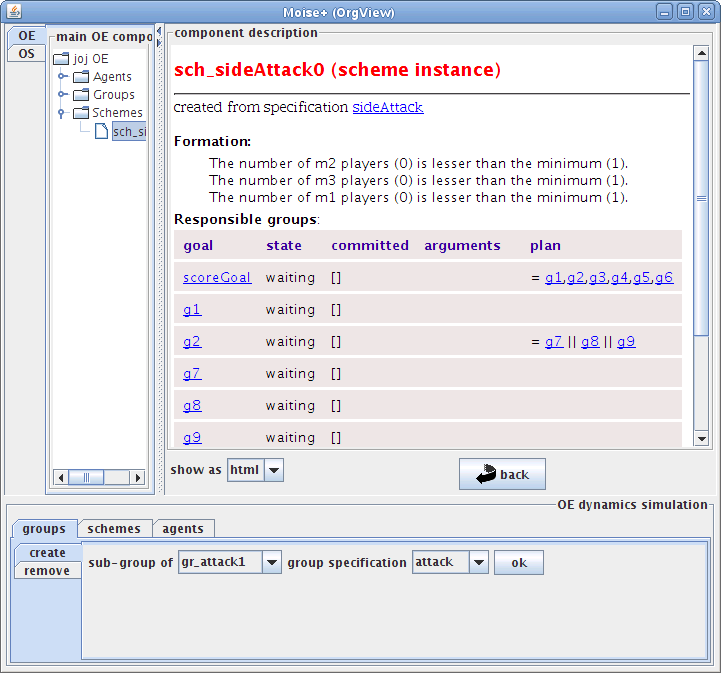
\includegraphics[width=.8\textwidth]{screens/sch1.png}
  \end{center}
  \caption{Scheme starting}
  \label{fig:sch1}
\end{figure}


\subsection{Goal state changes}

Each achievement goal of a scheme instance (as shown in the
\prettyref{fig:sch1}) has the following dynamic information:

\begin{enumerate}[$i$)]
\item state of the goal (possible states and the transitions are
  represented in \prettyref{fig:goal-states}). Every goal is initially
  \emph{waiting} the conditions to be pursued, when that condition is
  satisfied its state becomes \emph{enabled}.  For example, the goal
  $g_7$ is enabled only after the goal $g_1$ has been satisfied and thus
  before the $g_1$ satisfaction $g_7$ is in a waiting state. The
  \prettyref{alg:funcPreCond} specify when an goal becomes
  enabled. In the example of the \prettyref{fig:sch1} no goal is
  enabled since the scheme is not well formed yet. When the scheme is
  well formed, as shown in \prettyref{fig:sch1a}, only the goal $g_1$
  is enabled. As soon as $g_1$ is satisfied, the goals $g_7$, $g_8$, and
  $g_9$ becomes enabled (\prettyref{fig:sch2}). Once in the enabled state,
  the agents can pursue the goal and change its state to either
  satisfied or impossible. Goals without committed agents, pass from
  the state waiting to the state enabled/satisfied/impossible based on the
  satisfaction state of its sub-goals.

  The state of the goal can be changed in the `scheme'/`goal state' tab.


\item committed: a list of agents committed to this goal;
  
\item argument (a String): it is the values for the goal arguments
  (e.g. a value for the argument $M2Ag$ of the goal $g_3$).
  
\end{enumerate}


\begin{figure}[t]
  \begin{center}
    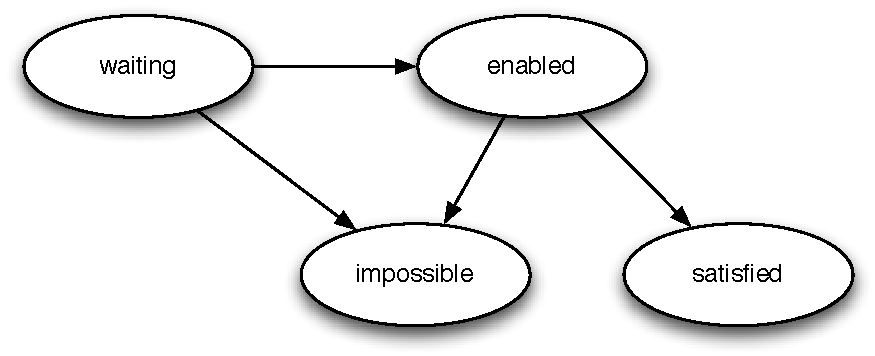
\includegraphics[width=0.8\textwidth]{figures/goal-states.pdf}
  \end{center}
  \caption{Goal states}
  \label{fig:goal-states}
\end{figure}


\begin{algorithm}[t]
\textbf{function} isEnabled(scheme $sch$, goal $g$)
~\\
~\\
\If{$sch$ {\rm is not well formed}}{
    \textbf{return} $false$\;
}
\If{$g$ {\rm has no committed agent}}{
    \textbf{return} $false$\;
}
\eIf{$g$ {\rm is the} $sch$ {\rm root}}{
    \textbf{return} $true$\;
}{
    $g$ {\rm is in a plan that match} `$g_0 = \cdots g \cdots$'\;
    \eIf{$g$ {\rm is in a plan that match} `$g_0 = \cdots g_i$ \textbf{,} $g \cdots$'}{
       \eIf{$g_i$ {\rm is already satisfied}}{
          \textbf{return} $true$\;
       }{
          \textbf{return} $false$\;
       }
    }{
       \textbf{return} isEnabled($sch$, $g_0$)\;
    }
}
\caption{Algorithm to verify possible goals}
\label{alg:funcPreCond}
\end{algorithm}

We have developed our soccer team organisation in two independent
dimensions of the \moise model: the structure and the functioning.
Since they are not linked yet, we can not create an agent with a role
and also a mission. Thus, the next section will explain how to link
these two dimensions.


% --------------------
\section{Normative Specification}

The \ac{NS} states both the required roles for missions and missions
obligations for roles. The \ac{SS} (\prettyref{sec:ss}) gives the
roles and the \ac{FS} (\prettyref{sec:fs}) gives the missions.

The \ac{NS} of our example is described in \prettyref{tab:jojDS}
and its specification in the XML file is simple:
{\small
\begin{verbatim}
<normative-specification>
   <norm id="n1" type="permission" role="back"     mission="m1" />
   <norm id="n2" type="obligation" role="middle"   mission="m2" />
   <norm id="n3" type="obligation" role="attacker" mission="m3" />
</normative-specification>
\end{verbatim}
}
% The lines 2--5 state the set of possible deontic operators, in the
% \moisem it is proposed two (\pode{} and \deve), but the user can extend
% it. The remaining lines describe the permissions/obligations of the
% roles exactly as proposed in \prettyref{tab:jojDS}.

From the point of view of simulation, this new OS allows us to create
an agent, assign to it a role (e.g.  attacker), and after a mission
(e.g. m3). From the point of view of the agent, if it 
\begin{enumerate}[$i$)]
\item adopts a role (e.g. attacker)
\item in a group responsible for an instance scheme (e.g. sch\_sideAttack0),
\item this role has obligations for some of this scheme's mission, and
\item the cardinality of this mission is not satisfied (i.e. the
  minimum number of agents committed to this mission is not achieved), 
\end{enumerate}
then it is obligated to commit to this mission (e.g. m3).

The next sections will exemplify how the scheme well formation status
and the agent obligations status may change according to the
agents commitments to missions.


\subsection{Responsible groups}

Each scheme has a set of responsible groups, agents from these groups
will perform the scheme. Therefore, only agents from these groups can
(or have to) commit to the missions of the scheme. Thus, the first step is
to add a responsible group for our scheme \texttt{sch\_sideAttack0}:
\begin{enumerate}
\item run the program \ldots/examples/tutorial/tutorialDS. This
  program creates an entity that already has the 11 agents, 3 groups,
  and 1 scheme as we had built in the previous sections.
  
\item In the OE tree, select the agent Roberto
  Carlos and notice that its obligations are Ok.
  
\item Select the `scheme'/`responsible groups' tab, select the
  scheme \texttt{sch\_sideAttack0}, and add the groups \group{gr\_attack1} and
  \group{gr\_defense2}. Notice how the Roberto Carlos's 
  obligations changed (\prettyref{fig:ds1}).

  \begin{figure}
    \begin{center}
      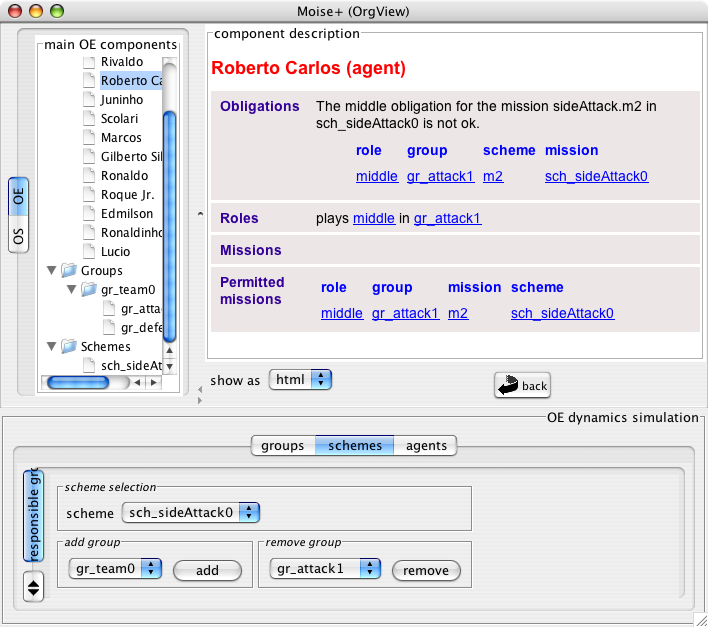
\includegraphics[width=.8\textwidth]{screens/ds1.png}
    \end{center}
    \caption{Agent obligations status}
    \label{fig:ds1}
  \end{figure}
  
\end{enumerate}

\subsection{Mission commitment}

The commitment to a mission is originated either by and agent's role
\emph{obligation} to the mission or by an agent own interest in the
mission. In the latter case, the agent must have a role that gives it
the \emph{permission} for the mission. For example, the player
Roberto Carlos can commit to the mission m2 since its middle role in
the \group{gr\_attack1} gives him permission\footnote{Indeed, this
  role gives obligation for the missions, but all obligation is
  also a permission.} to this mission.

To practice this event, try the following:
\begin{itemize}
\item select the `agent'/`missions' tab, select the agent
  `Roberto Carlos', select the mission `m2', and click on the
  `ok' button. Notice that the Roberto Carlos obligation status
  becomes ok. But the sch\_sideAttack0 is not well formed yet.
\item Commit the agent Ronaldo to the mission m3.
\item Commit the agent Lucio to the mission m1. The sch\_sideAttack0 is
  now well formed (\prettyref{fig:sch1a}).

\item Try to commit the agent Rivaldo (an attacker) to the mission m1.
\item Try to commit the agent Edmilson (a back) to the mission m1.
\item Try to commit the agent Marcos (the goal-keeper) to the mission
  m1. Notice that the Marcos is allowed to the mission m1 since
  goal-keeper is a back sub-role and back is permitted to m1. Thus the
  error is about the cardinality of the mission m1.
\end{itemize}

\begin{figure}
  \begin{center}
    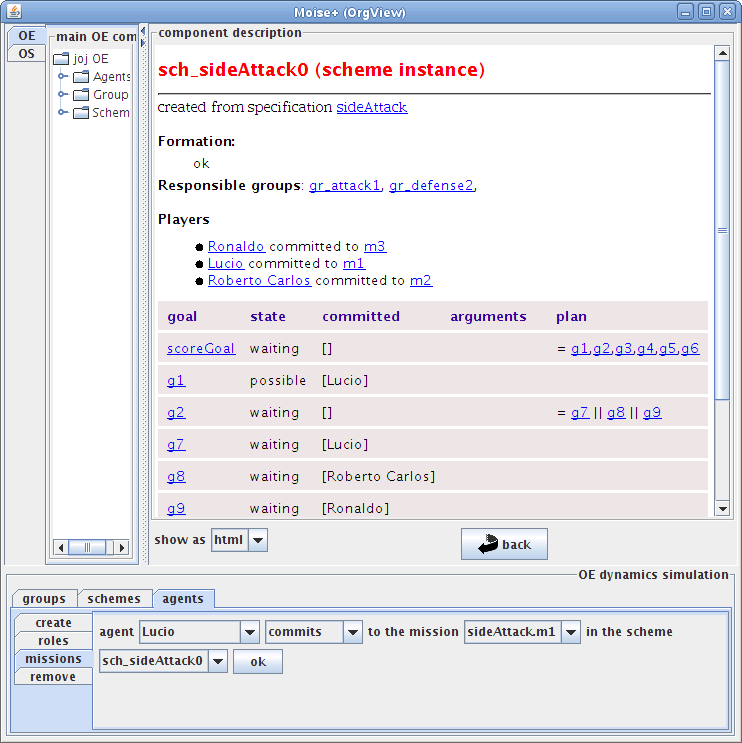
\includegraphics[width=.8\textwidth]{screens/sch1a.png}
  \end{center}
  \caption{Scheme well formed}
  \label{fig:sch1a}
\end{figure}


\begin{figure}
  \begin{center}
    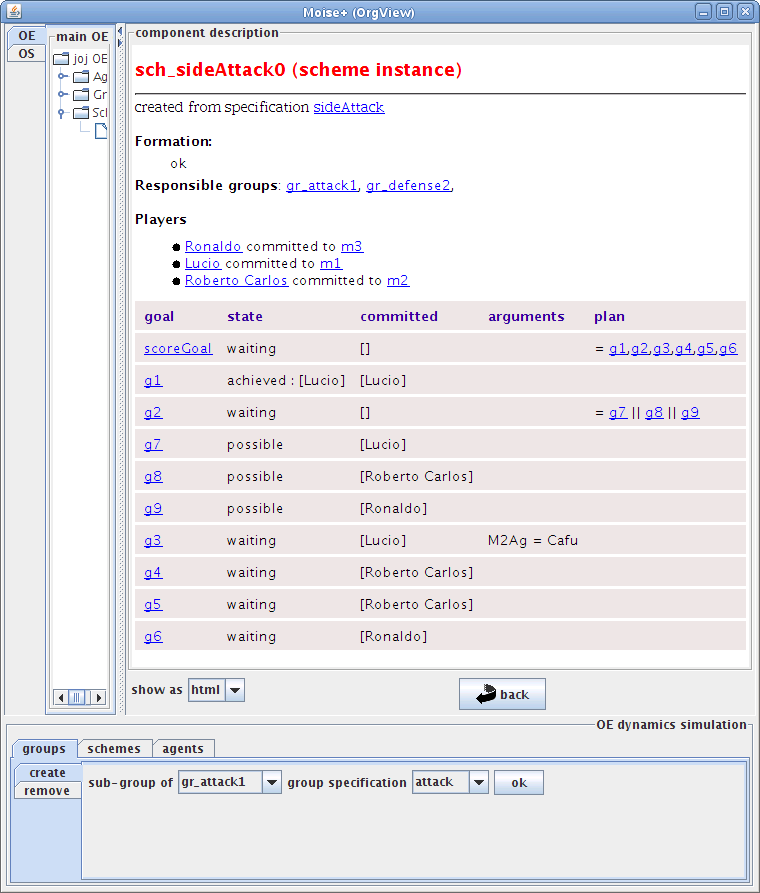
\includegraphics[width=\textwidth]{screens/sch2.png}
  \end{center}
  \caption{Scheme with goal $g_1$ achieved}
  \label{fig:sch2}
\end{figure}


% --------------------
\section{Entity de-construction}

We have build a well formed OE in the previous sections. Now select
the `group'/`remove' tab and try to remove the gr\_team0. You will
realize that there are many constraints for the remotion of any OE
element. For example, to remove a group, the group must have no
players; to remove a group player, the player must play no role in it;
to remove a player's role, the role must not be necessary for some
player's mission, etc. The \prettyref{fig:remOE} shows these
dependencies.
%  and the file \ldots/moise/doc/oeEvents/index.html describes
% the constrains for each event.

\begin{figure}
  \begin{center}
    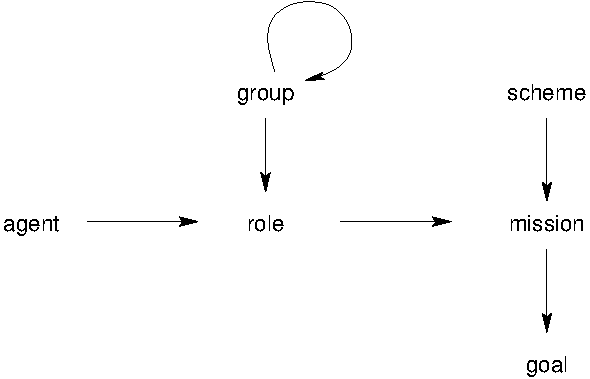
\includegraphics[width=.6\textwidth]{figures/remDynamics.pdf}
  \end{center}
  \caption{Dependence for deletion}
  \label{fig:remOE}
\end{figure}



%
%  Saci
%  ---------
%

\appendix

\chapter{Developing Organised Agents with \jmoisem}
\label{chp:jmoisem}

This chapter describes an example of a simple MAS composed by agents
that are aware of its organisation. These agents are developed with
\jmoisem which is based on \Jason, an interpreter used to program BDI
agents (\url{http://jason.sf.net}, \cite{bordini:07}). \jmoisem is
very similar to \smoisem (appendix~\ref{chp:smoise}) regarding the
overall system concepts (e.g. OrgManager and OrgBox components). The
main difference is how the agents are programmed, in \smoisem agents
are programmed in Java (using a very simple agent architecture), while
in \jmoisem they are programmed in AgentSpeak, a programming language
based on BDI concepts and thus more suitable for agents programming.

\begin{quote}
\textsc{Note:} The \Jason \moisem integration was changed when we moved to ORA4MAS
platform. However, the concepts, from an agent perspective, are the same. So we
leave the chapter in this tutorial. Refer to \texttt{doc/ora4mas} for
the current programming proposal.  
\end{quote}

The next section describes how we have customised the \Jason agent
architecture to enable agents to perceive and reason about its
organisation. It is described from an user point of view and no implementation
issues are therefore given (a more detailed description of \jmoisem was
published in \cite{hubner:07}). The \prettyref{sec:agWP-jason} exemplifies the
use of \jmoisem in the application described in \prettyref{sec:exeWP}.

\section{Organisational agent architecture in \Jason} \label{sec:jArc}

In \jmoisem an agent changes its organisation using organisational
actions and perceives it back by organisational events.

\begin{figure}
  \begin{center}
    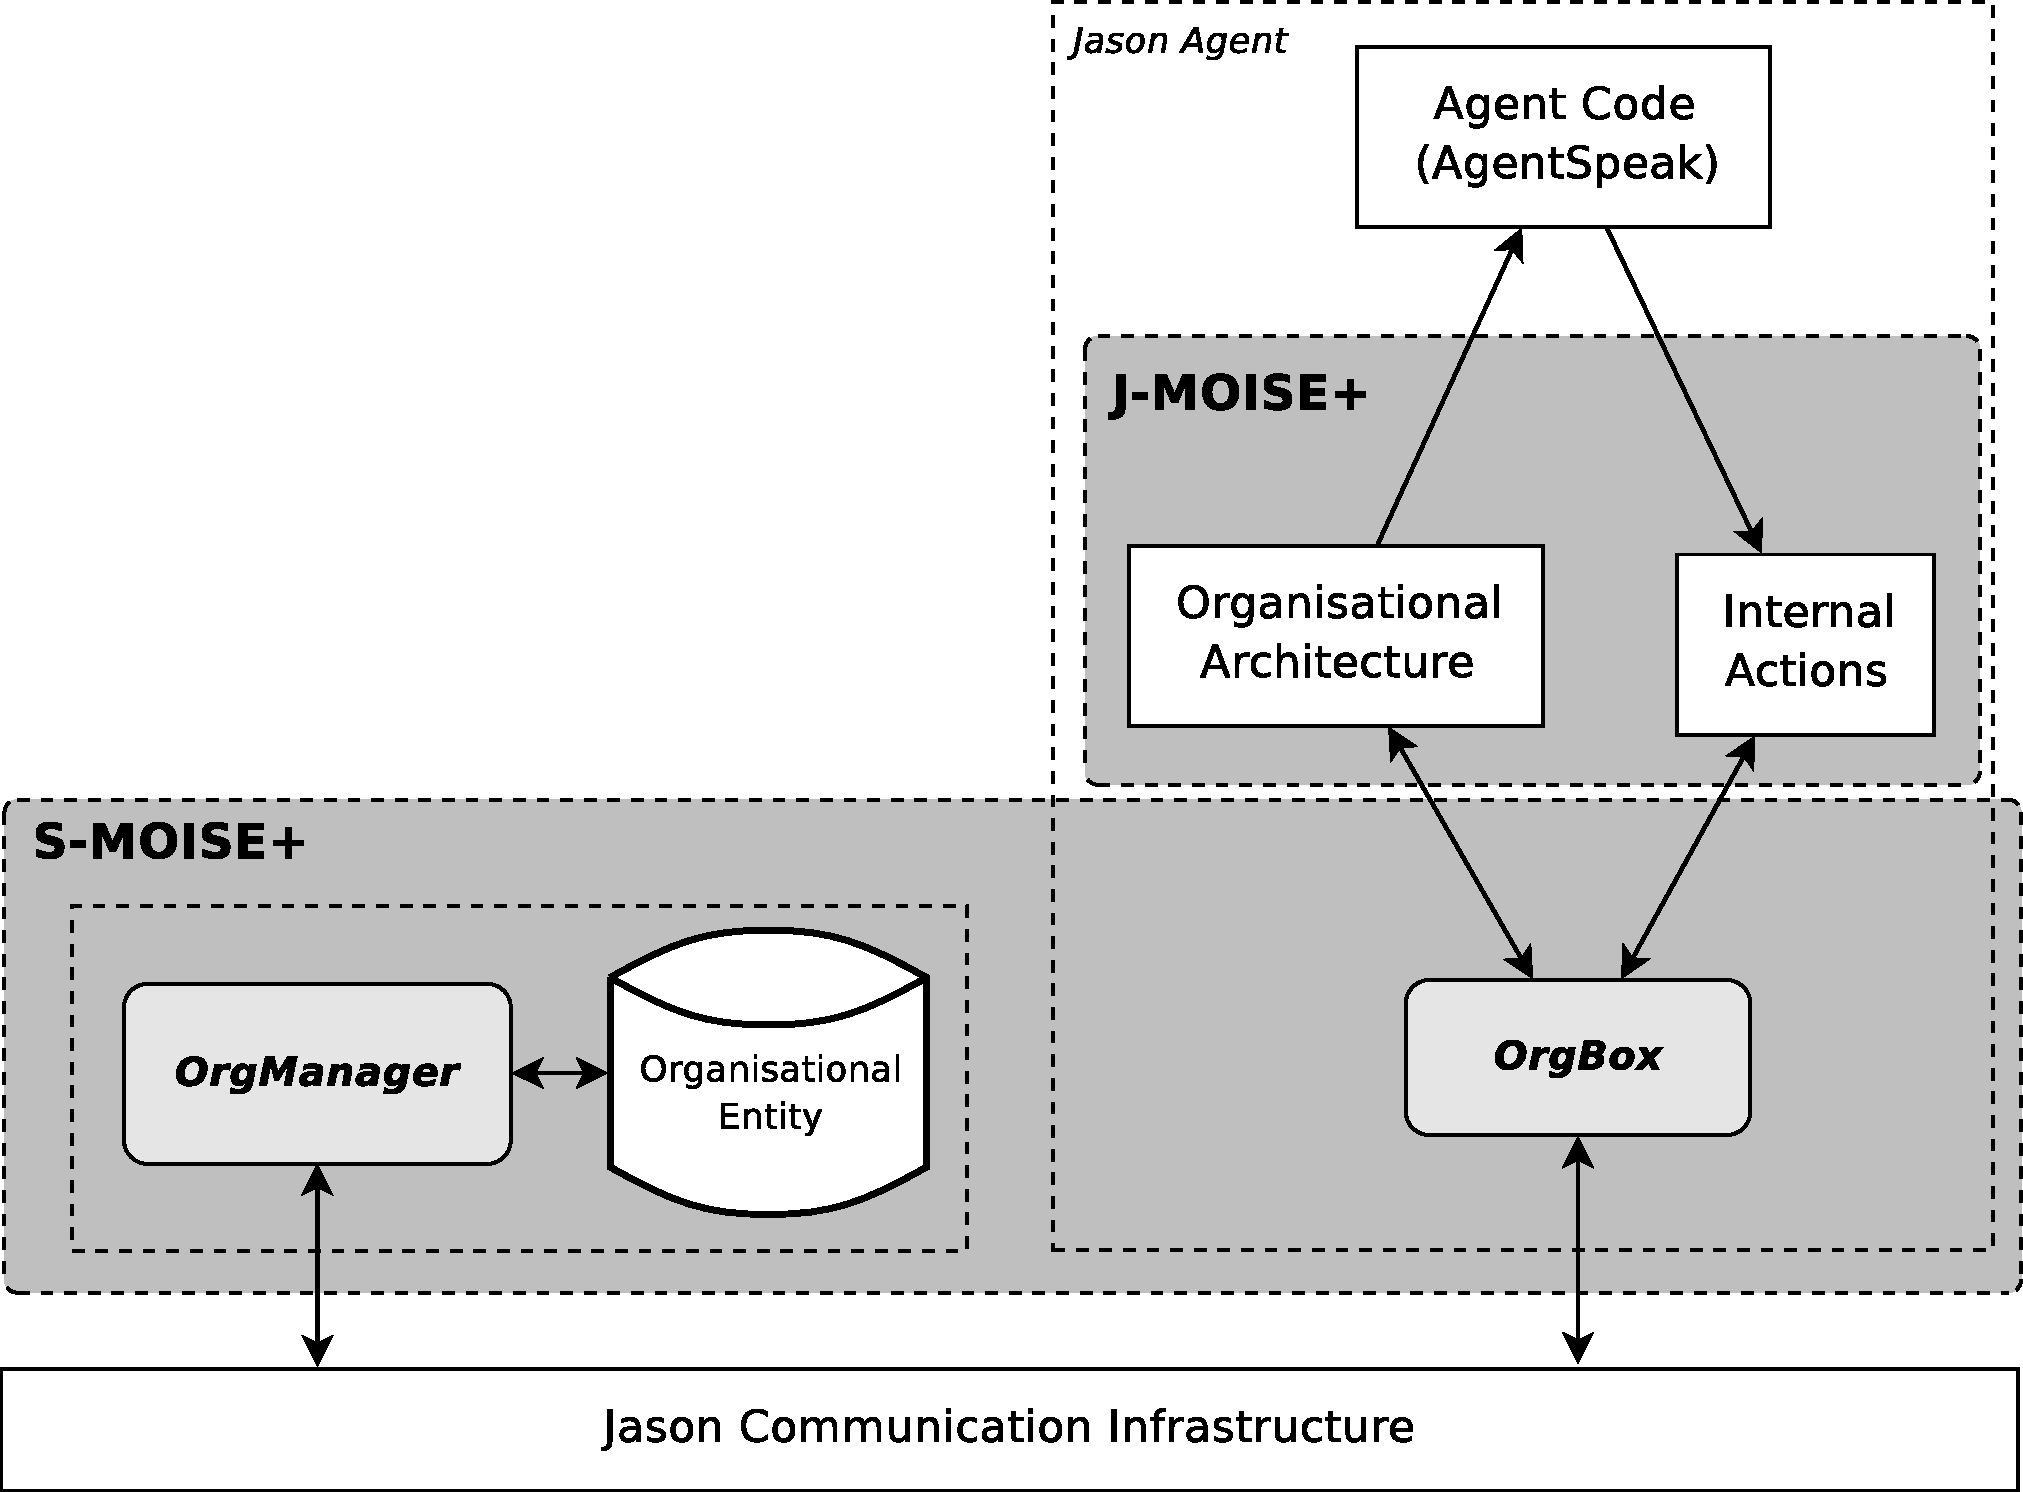
\includegraphics[width=.9\textwidth]{figures/jmoise-general.pdf}
  \end{center}
  \caption{General view of the \jmoisem architecture}
  \label{fig:jmoise}
\end{figure}

\subsection{Organisational actions}

The overall proposal is based on the addition of a special agent
called OrgManager that maintains the current organisational entity
(OE) state \cite{hubner:05a} (see \prettyref{fig:jmoise}). The agents
then may send messages to OrgManager, using \Jason communication acts,
to produce \emph{actions} that change the OE. For example, to create a
new group from the specification \group{wpgroup} (see
\prettyref{sec:exeWP}), an agent should send an achieve message with
content \texttt{create\_group(wpgroup)} to the agent called
orgManager\footnote{\texttt{.send} is the \Jason internal action used
  to send messages to another agent.}:

\begin{verbatim}
  +some_event : true 
     <- .send(orgManager, achieve, create_group(wpgroup)).
\end{verbatim}
% In this example the performative \texttt{askOne} is used since the
% agent wants a response with the new group identification (the response
% will unifies with the \texttt{GId} variable). However, in the case
% where some agent is not concerned with the result of the message, it
% can use the \texttt{achieve} performative:

% \begin{verbatim}
%   +someEvent : true 
%      <- .send(orgManager, achieve, createGroup(wpgroup)).
% \end{verbatim}

It is also possible to use an organisational action in the plan using
the \jmoisem internal actions that sends the corresponding message to
OrgManager (these actions start with \texttt{jmoise.}), for example:

\begin{verbatim}
  +some_event : true 
     <- jmoise.create_group(wpgroup).
\end{verbatim}


The actions that OrgManager can handle are\footnote{These actions
  correspond to the organisational actions described in
  \prettyref{chp:simulator}.} \footnote{A detailed explanation and
  examples are found in \href{http://moise.sf.net/doc/jmoise/api}{API documentation} of \jmoisem.}:
\begin{itemize}

\item \texttt{create\_roup(<GrSpecId>[,<GrId>])}: creates a new group instance
  based on GrSpecId specification. To create a subgroup, the super group
  identification must be informed as the second argument.\footnote{More
    arguments can be used to define the identification of the new group or
    obtain the automatically given identification (see API for more
    information about these arguments).}

\item \texttt{remove\_group(<GrId>)}: removes the group identified by
  GrId, this groups must be empty (no players) to be removed.

\item \texttt{create\_scheme(<SchSpecId> [, <ListOfRespGr>])}: creates a new
  scheme instance based on scheme specification identified by SchSpecId. If
  the second optional parameters is used, the initial set of responsible
  groups of the new scheme is defined by ListOfRespGr.

\item \texttt{add\_responsible\_group(<SchId>,<GrId>)}: add the group
  GrId as responsible group for scheme SchId.

%\item \texttt{remove\_responsible\_group(<SchId>,<GrId>)} *

\item \texttt{remove\_scheme(<SchId>)}: removes the scheme SchId from
  the OE.

\item \texttt{abort\_scheme(<SchId>)}: removes the scheme SchId from
  the OE (does not requires that the scheme has no players).

\item \texttt{set\_goal\_arg(<SchId>,<Goal>,<ArgId>,<value>)}: set an
  argument's value for some goal in a scheme.

\item \texttt{set\_goal\_state(<SchId>,<Goal>,(satisfied|impossible))} 

%\item \texttt{addAgent()}
%\item \texttt{removeAgent()} *

\item \texttt{adopt\_role(<RoleId>,<GrId>)}: adopts the role RoleId in
  the group GrId.

\item \texttt{remove\_role(<RoleId>,<GrId>)}: removes the role RoleId
  in group GrId.

\item \texttt{commit\_mission(<MisId>,<SchId>)}: commit the agent to
  mission MisId in scheme SchId.

\item \texttt{remove\_mission([<MisId>,] <SchId>)}: if MisId is not
  informed, all missions in the SchId will be removed.

\item \texttt{broadcast( <GrpId/SchId>, P, C)}: broadcast a message with
  content C and performative P to all agents of a group or scheme.
\end{itemize}

\noindent
You can see the API documentation for a complete list of actions, more
details, and examples.

\subsection{Organisational events}

The \Jason programmer may customise several components of the system,
in the \jmoisem we customise the agent architecture that is
responsible to link the agent to its environment and the other
agents. We particularly change the agent perception to include
\emph{organisational events}, the agent thus perceive when a group is
created, when a scheme is started, when it has an organisational
obligation, and so on. For example, when a new group is created, the
event \texttt{+group(<GrSpecId>, <GrId>)} is added in the set of
perceptions of the agent and it can handle this event with plans like
the following:
\begin{verbatim}
  +group(wpgroup,Id) : true
     <- jmoise.adopt_role(writer,Id).
\end{verbatim}
In this example, whenever a group from specification \group{wpgroup}
is created, the agent adopts the role \role{writer}. Of course the
plan context (\texttt{true} in above example) may constrain the role
adoption. For instance, in the following plan, the agent only adopts
the role in case the group creator is its friend
\begin{verbatim}
  +group(wpgroup,Id)[owner(O)] : my_friend(O)
     <- jmoise.adopt_role(writer,Id).
\end{verbatim}

The events which start with \texttt{+} represent a belief
addition. However when, for example, a group is removed from the
organisational entity, a belief deletion event is generated. In this
case, the event is \texttt{-group(<GrSpecId>, <GrId>)} and it can be
handle by plans like:
\begin{verbatim}
  -group(wpgroup,Id) : true
     <- .print("The group ",Id," was removed!").
\end{verbatim}



The events perceived by the agent are the following: 

\begin{itemize}
\item \texttt{+/- group(<GrSpecId>,<GrId>)[owner(<AgName>)]}:
  perceived by all agents when a group is created (event \texttt{+})
  or removed (event \texttt{-}) by \texttt{AgName}.

\item \texttt{+/- play(<AgName>, <RoleId>, <GrId>)}: perceived by the
  agents of \texttt{GrId} when an agent adopts (event \texttt{+}) or
  remove (event \texttt{-}) a role in group \texttt{GrId}.

\item \texttt{+/- commitment(<AgName>, <MisId>, <SchId>)}: perceived
  by the \texttt{SchId} players when an agent commits or removes a
  commitment to a mission \texttt{MisId} in scheme \texttt{SchId}.

\item \texttt{+/- scheme(<SchSpecId>,<SchId>)[owner(<AgName>)]}:
  perceived by all agents when a scheme is created (\texttt{+}),
  finished (\texttt{-}), or aborted (\texttt{-}) by \texttt{AgName}.

\item \texttt{+ scheme\_group(<SchId>,<GrId>)}: perceived by
  \texttt{GrId} players when this group becomes responsible for the
  scheme \texttt{SchId}.

\item \texttt{+ sch\_players(<SchId>,<NumberOfPlayers>)}: perceived only
  by the owner of the scheme when the number of players changes
  (agents commit or remove a commitment in the scheme).

\item \texttt{+ goal\_state(<SchId>, <GoalId>, <State>)}: perceived by
  \texttt{SchId} players when the state of some goal changes.

\item \texttt{+/- obligation(<SchId>, <MisId>)[role(<RoleId>),
    group(<GrId>)]}: perceived by an agent when is has an
  organisational obligation for a mission. It has a role
  (\texttt{RoleId}) in a group (\texttt{GrId}) responsible for a
  scheme (\texttt{SchId}) and this role is obligated to a mission in
  this scheme.

\item \texttt{+/- permission(<SchId>, <MisId>)[role(<RoleId>),
    group(<GrId>)]}: perceived by an agent when is has an
  organisational permission for a mission. It has a role
  (\texttt{RoleId}) in a group (\texttt{GrId}) responsible for a
  scheme (\texttt{SchId}) and this role has permission to a mission in
  this scheme.

\end{itemize}

The agent architecture also generate goal achievement events when an
agent's organisational goals becomes possible in the current state of
the scheme execution. The programmer can thus write plans to deal with
these events to enable to agent to achieve its organisational
goals. For example, when the goal to write the paper conclusion is
permitted, the following plan will be executed:
\begin{verbatim}
  +!wconc[scheme(Sch)] : true 
     <- .print("Writing the conclusion!");
        jmoise.set_goal_state(Sch, wconc, satisfied).
\end{verbatim}
The \texttt{[scheme(Sch)]} in the plan's trigger event represents a set of
annotations of the goal (only one annotation in this case). Differently than
arguments (enclosed by `(' and `)'), annotations may not be included in the
predicate. The above plan can thus simply be:
\begin{verbatim}
  +!wconc : true 
     <- .print("Writing the conclusion!");
        // obtain the scheme id from the belief base
        ?scheme(writePaperSch, Sch); 
        jmoise.set_goal_state(Sch, wconc, satisfied).
\end{verbatim}
Of course, in place of printing a message the plan should have action
that achieve the goal. Note that when the goal is achieved, the agent
have to notify the OrgManager, so it can change the state of the
scheme execution and coordinate its execution. If the goal is not
achieved, the OrgManager also have to be notified, for instance:
\begin{verbatim}
  +!wconc[scheme(Sch)] : true 
     <- .print("Writing the conclusion!");
        jmoise.set_goal_state(Sch, wconc, satisfied).
  // the plan to achieve the goal failed 
  -!wconc[scheme(Sch)] : true 
     <- jmoise.set_goal_state(Sch, wconc, impossible).
\end{verbatim}

Other annotations of goals events are:
\begin{itemize}
\item \texttt{mission(MissionId)}: the mission of the goal;
\item \texttt{type(Type)}: the type of the goal (achievement or maintenance);
\item \texttt{source(orgManager)}: the source of the goal, always the
  orgManager in case of organisational goals;
\item \texttt{role(RoleId)}: the role assigned to the mission of the goal;
\item \texttt{group(GrpId)}: the group where the role is being played.
\end{itemize}
The plan may add these annotation if the corresponding information is
necessary for the execution of the plan, for example:
\begin{verbatim}
  +!wconc[scheme(Sch), role(R), group(G)] : true 
     <- .print("Writing the conclusion for the scheme ",Sch);
        .print("because I play ",R," in group ",G);
        ...
\end{verbatim}

%\subsection{Internal Actions}

%.hasAuthority(<AgName>,<AgName>)


\section{The writing paper agents in AgentSpeak}
\label{sec:agWP-jason}

In this section, the write paper application (as presented in
\prettyref{sec:exeWP}) is implemented using AgentSpeak and \Jason. 

\subsection{MAS2J configuration}

Projects in \Jason are defined in a \texttt{.mas2j} configuration
file. In this file we set which agents will run and some parameters
for these agents. The write paper application is composed by the
following agents:
\begin{itemize}
\item OrgManager: this agent is the same as presented in the \smoisem,
  but customised to provide organisational services in \Jason
  systems. 
\item Jaime: this agent will play the editor role in the application.
\item Olivier: this agent will play the writer role.
\item Jomi: this agent will also play the writer role.
\end{itemize}
All agents have a customised architecture (as depicted in
\prettyref{fig:jmoise}) that bind them to the organisational
infrastructure. The OrgManager has two special parameters: the XML
file with the organisational specification and whether the a graphical
interface will be shown. In the specification of the organisation, the
user must start all identifiers with \textbf{lower case} characters,
since identifiers that start with upper case are considered as
variables in AgentSpeak.

{\footnotesize
\verbatiminput{\wpjason/writePaper.mas2j}
}

\subsection{Jaime's code}
{\footnotesize
\verbatiminput{\wpjason/jaime.asl}
}

\noindent
The included file (\texttt{moise-common.asl}) is:
{\footnotesize
\verbatiminput{jmoise/src/asl/moise-common.asl}
}


\subsection{Olivier's code}
{\footnotesize
\verbatiminput{\wpjason/olivier.asl}
}

\subsection{Jomi's code}
{\footnotesize
\verbatiminput{\wpjason/jomi.asl}
}

\subsection{Execution}
\begin{verbatim}
[jaime]   Writing title!
[jaime]   Writing abstract!
[jaime]   Writing section titles!
[jomi]    Writing sections!
[olivier] Doing organisational goal wsecs in scheme sch_writePaperSch0
[jaime]   Writing conclusion!
[olivier] Doing organisational goal wrefs in scheme sch_writePaperSch0
[jaime] ***** FINISH! *****
... continue with next paper ...
\end{verbatim}

\subsection{Screen shots}

The following screen is the mind of the Jaime agent after the
execution of the write paper scheme.
\begin{center}
  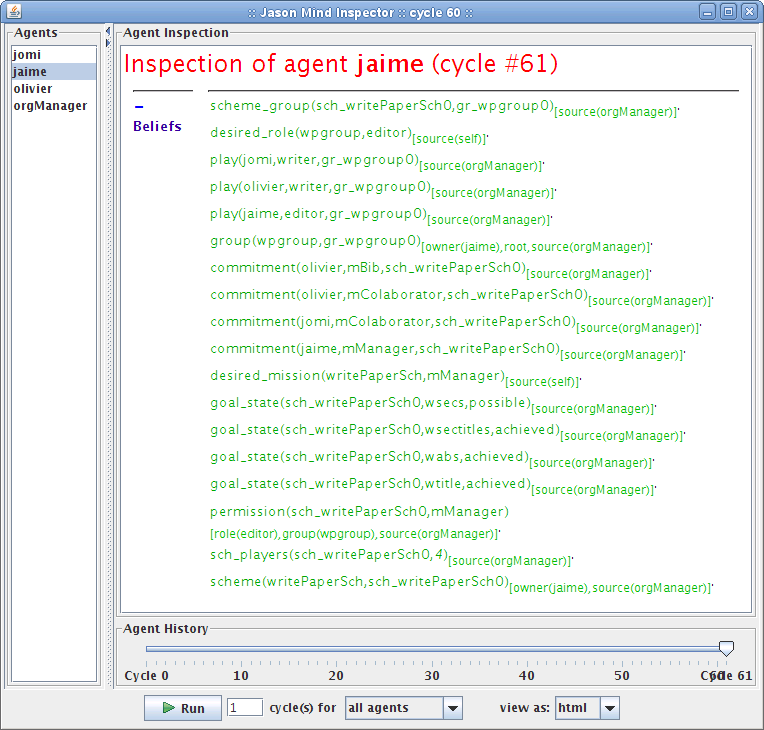
\includegraphics[width=\textwidth]{screens/jaimeMind.png}
\end{center}

\newpage
\noindent
The screen below is the status of the write paper scheme in the end of
the execution.
\begin{center}
  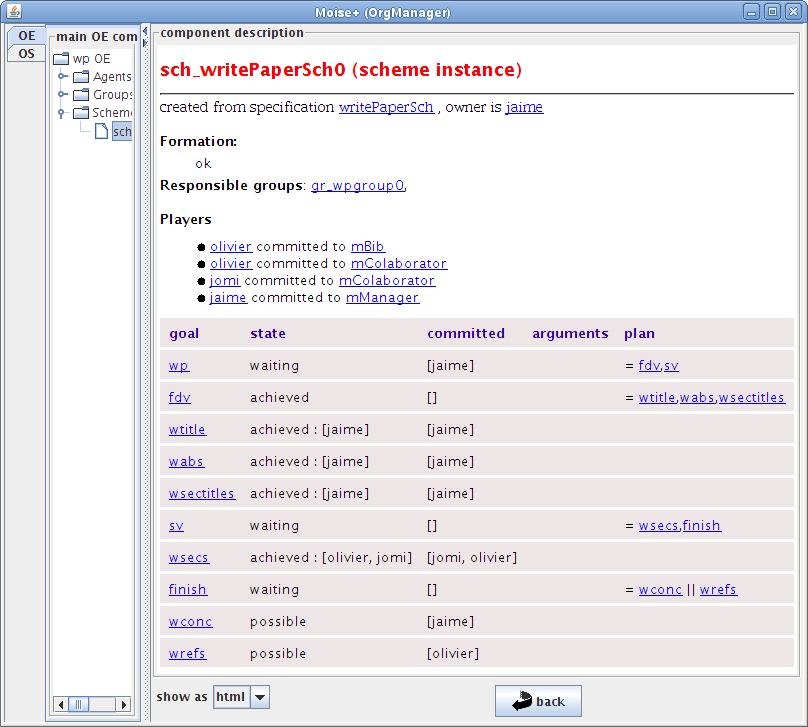
\includegraphics[width=\textwidth]{screens/jmoise-scheme-status.png}
\end{center}
  


\chapter{Developing Distributed Organised Agents with \smoisem} \label{chp:smoise}

This chapter describes an example of a simple MAS composed by
distributed agents that follows an organisational specification. These
agents are developed with \smoisem, an extension to \saci
(\url{http://www.lti.pcs.usp.br/saci}) where the agents have an
organisational aware architecture. This tool is proposed in
\cite{hubner:05a} (this paper is available in the publications
directory of the \moisem distribution). While the paper focus on the
organisation framework, this chapter focus on the agents
development. Thus the next section describes a simple architecture for
organised agents and \prettyref{sec:agWP} explains how this
application agents could be developed.\footnote{As remarked in the
  introduction, this tool is not supported anymore. Refer to
  \texttt{doc/ora4mas} for the current programming proposal.}

\section{A simple organisational agent architecture} \label{sec:soArc}

The proposed architecture is very simple and is just a starting point 
towards organisation oriented programming. The base idea is an agent
that always do what its organisation needs, it does not have personal
goals, and thus there is no conflict between goals.

The following algorithm summarises the agent functioning cycle:
\begin{center}
\begin{algorithm}[H]
\While{true}{
    $g \gets $ choseGoal()\;
    $p \gets $ makePlan($g$)\;
    execute($p$)\;
}
\end{algorithm}
\end{center}
The agent firstly chooses an organisational goal, plans a sequence of
actions to achieve it, and then executes the plan. \textsf{MakePlan} and
\textsf{execute} are domain dependent, whereas \textsf{choseGoal}
function is general and could be
\begin{center}
\begin{algorithm}[H]
\textbf{function} choseGoal() : Goal\;
\If{there is an organisational goal permitted to be achieved}{
    returns it\;
}
\If{I have no role}{
    adopts a role\;
    returns choseGoal()\;
}
\If{try to commit to an obligated mission}{
    returns choseGoal()\;
}
\If{try to commit to a permitted mission}{
    returns choseGoal()\;
}
\If{try to uncommit to finished schemes}{
    \For{all mission $m$ I am committed to}{
        \If{the scheme of $m$ is already finished}{
           uncommit($m$)\;
         }
    }
}
returns no goal\;
\end{algorithm}
\end{center}

According to this algorithm, in case the agent has no organisational goal
(first if), it firstly tries to adopt a role, then tries to commit to an
obligated mission, and lastly it tries to commit to a permitted mission. After
its commitments, it eventually will get an organisational goal. The last
\textbf{if} remove the agent commitments when a scheme are already
finished. Note that this algorithm assumes that the agent will enact only one
role in the organisation.


\section{The write paper agents}\label{sec:agWP}


The \smoisem API has three main classes to access the organisational
layer (as defined in \cite{hubner:05a}): 
\begin{itemize}
\item \textsf{OrgBox}: this class has methods to generate
organisational events like role adoption, mission commitment, group
creation, etc. (See the \href{../api/saci/moise/package-summary.html}{API
documentation} for a detailed documentation).

\item \textsf{OEAgent}: this class represents the agent inside the
organisation, it stores the agents roles, missions, etc.

\item \textsf{BaseOrgAgent}: this class implements the architecture
described in \prettyref{sec:soArc}. It has two attributes
\textsf{currentGoal} (from class \textsf{GoalInstance}) and
\textsf{currentPlan} (a Java \textsf{List}). \textsf{currentGoal} is
initialised in the \textsf{choseGoal} method and \textsf{currentPlan}
is initialised in the user's \textsf{plan} method. The
\textsf{currentPlan} is a list of strings where each element is an action
description.

\end{itemize}

Using these classes, it is quite easy to code agents in the \smoisem
framework. The programmer needs to override the \textsf{adoptRole},
\textsf{plan}, and
\textsf{executeAct} methods of the \textsf{BaseOrgAgent} class. For
example, the Jomi agent program is\footnote{The
code for exceptions handling is omitted to increase readability.}:

{\footnotesize
\begin{verbatim}
public class JomiAg extends BaseOrgAgent {

    public static void main(String[] args) {
        JomiAg a = new JomiAg();

        if (a.enterSoc("jomi", "writePaperSoc")) {
            a.initAg(null);
            a.run();
        }
    }

    protected boolean adoptRole() {
        String roleId = "writer";
        String grTeamId = getOrgBox().getRootGroupInstance( "wpgroup" );
        if (grTeamId != null) {
            getOrgBox().adoptRole(roleId, grTeamId);
            print("adopted the role "+roleId);
            return true;
        } else {
            print("plan aborted: can not identify/create a group team");
        }
        return false;
    }

    protected void plan() {
        currentPlan = null;
        if (currentGoal != null) {
            // create a plan that only prints the current goal!
            currentPlan = new ArrayList();
            currentPlan.add("print("+currentGoal+")");
        }
    }

    protected void executeAct(String action) {
        if (action.startsWith("print"))
            print(action);
   }
}
\end{verbatim}
}

The \textsf{main} method just creates an \textsf{JomiAg} instance,
enter this agent in the society, and runs it. The default run method
is the one proposed in the architecture (a while true loop).

When the \textsf{choseGoal} method do not find an organisational goal for
the agent, it first calls \textsf{adoptRole}. This Jomi's method gets
the identification of the \group{wpgroup}
instance\footnote{In case where there is
no instance, the \textsf{getRootGroupInstance} method creates one.}
 and adopts the `writer' role in this group.

Jomi's \textsf{plan} method is very simple, itcreates a plan
with only one action that is to print the goal! Having a plan, the
architecture calls \textsf{executeAct} for each action of the
current plan. Finally the \textsf{executeAct} method executes the
print actions.

The Jaime program is:
{\footnotesize
\begin{verbatim}
public class JaimeAg extends BaseOrgAgent {

    public static void main(String[] args) {
        JaimeAg a = new JaimeAg();

        if (a.enterSoc("jaime", "writePaperSoc")) {
            a.initAg(null);
            a.run();
        }
    }

    protected boolean adoptRole() {
        String roleId = "editor";
        String grTeamId = getOrgBox().getRootGroupInstance( "wpgroup" );
        if (grTeamId != null) {
            getOrgBox().adoptRole(roleId, grTeamId);
            print("adopted the role "+roleId);
            return true;
        } else {
            print("plan aborted: can not identify/create a group team");
        }
        return false;
    }

    protected void uncommit(MissionPlayer mp) {
        super.uncommit(mp);

        // it is the case my scheme is finished
        SCH schWP = findSch();
        if (schWP != null) {
            if (schWP.getRoot().isSatisfied()) {
                getOrgBox().finishSCH(schWP.getId());
                destroy(); // kill myself
            }
        }
    }
	
    protected void plan() {
        currentPlan = null;
        if (currentGoal == null) { // there is no goal
            // create a Write a Paper scheme
            if (findSch() == null) 
               createSch();
            choseGoal();
        } 
        if (currentGoal != null) {
           // create a plan that only prints the current goal!
           currentPlan = new ArrayList();
           currentPlan.add("print("+currentGoal+")");
        }
    }
	
    protected void executeAct(String action) {
        if (action.startsWith("print"))
           print(" * doing * "+action);
    }

    SCH findSch() {
        // find my group scheme
        Group myGroup = getRolePlayer().getGroup();
            
        Iterator iSch = getOrgBox().getOE().
               findInstancesOfSchSpec( "writePaperSch" ).iterator();
        while (iSch.hasNext()) {
            SCH sch = (SCH)iSch.next();
            if (sch.getResponsibleGroups().contains( myGroup ))
                return sch;
        }
        return null;
    }
    
    boolean firstSchAlreadyCreated = false;
    SCH createSch() {
       if (firstSchAlreadyCreated)
          return null;

       String schId = getOrgBox().startSCH( "writePaperSch" );
       // set the responsible group
       getOrgBox().addResponsibleGroup(schId, getRolePlayer().
                                       getGroup().getId() );
       firstSchAlreadyCreated = true;
       return getOrgBox().getOE().findSCH(schId);
    }
    
    public RolePlayer getRolePlayer() {
       return (RolePlayer)getOrgBox().getMyOEAgent().
              getRoles().iterator().next();
    }    
}
\end{verbatim}
}

This agent planner creates a write paper scheme in case it could not
find an organisational goal (chose goal equals null). It also overrides
the \textsf{uncommit} method. If Jaime uncommits its $mMan$ mission,
it means that the root goal of the write paper scheme is achieved, and
thus Jaime can finish the scheme (remove it from the organisational
entity). Since a scheme could be finished only when
it has no players, Jaime waits that other agents uncommit and then
finishes the scheme. 

The following steps describe how to run this MAS with Ant
scripts\footnote{You need to install Ant to run this example as
described here, it is available at \url{ant.apache.org}.}:
\begin{enumerate}
\item Go to \texttt{saci/examples/moise/writePaper} directory

\item Start Saci
\begin{verbatim}
  ant saci
\end{verbatim}

\item Start the OrgManager. In the Saci window,
menu Launcher/Start Societies, fill the fields as shown in the figure
below.
  \begin{center}
    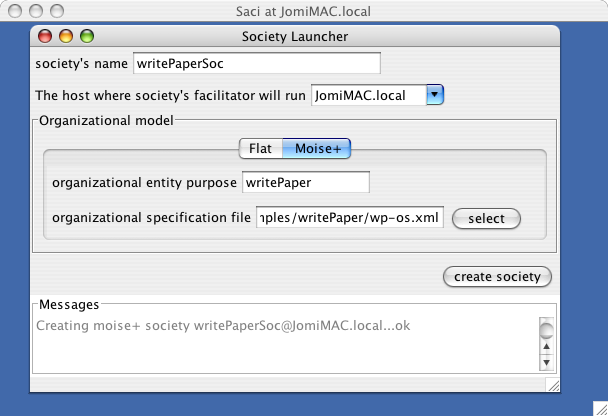
\includegraphics[width=.8\textwidth]{screens/createWPSoc.png}
  \end{center}
  
Alternatively, start the OrgManager by Ant
\begin{verbatim}
  ant orgManager
\end{verbatim}

The OrgManager will create a new window where the current
organisational specification and entity can be consulted.

  \begin{center}
    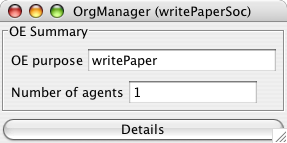
\includegraphics[width=.5\textwidth]{screens/orgManager.png}
  \end{center}
 
\item Run the Jaime agent
\begin{verbatim}
  ant jaime
\end{verbatim}
The output should be something like:
{\small
\begin{verbatim}
Agent jaime is inside society writePaperSoc
[jaime] adopted the role editor
[jaime] committed to permitted mission writePaperSch.mManager
        in sch_writePaperSch0 [jaime] my goal is wtitle
[jaime] Executing plan [print(wtitle)]
[jaime]  * doing * print(wtitle)
[jaime] Setting wtitle as satisfied.
[jaime] my goal is wabs
[jaime] Executing plan [print(wabs)]
[jaime]  * doing * print(wabs)
[jaime] Setting wabs as satisfied.
[jaime] my goal is wsectitles
[jaime] Executing plan [print(wsectitles)]
[jaime]  * doing * print(wsectitles)
[jaime] Setting wsectitles as satisfied.
[jaime] my goal is fdv
[jaime] Executing plan [print(fdv)]
[jaime]  * doing * print(fdv)
[jaime] Setting fdv as satisfied.
\end{verbatim}
}

Note that Jaime adopted the \role{editor} role, committed to $mMan$
mission and satisfied the goal \goal{fdv} (first darft version).

%The current scheme state is depicted in the
%\prettyref{fig:wpSchState}. This screen is shown when the Details
%button of the OrgManager is clicked.

%\begin{figure}
%  \begin{center}
%    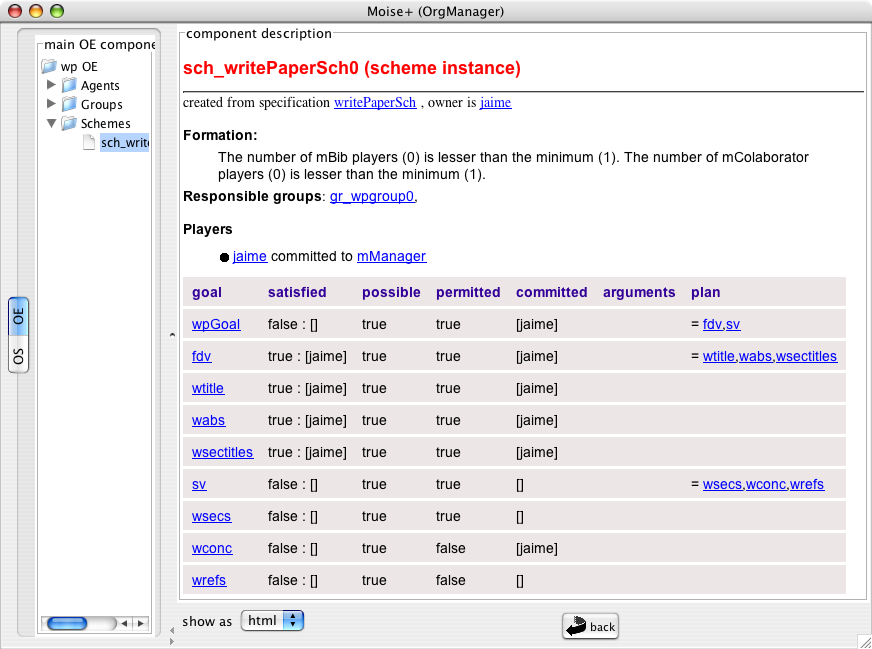
\includegraphics[width=.7\textwidth]{screens/writePaperSch.png}
%  \end{center}
%  \caption{The write paper scheme state}
%  \label{fig:wpSchState}
%\end{figure}



\item Run the Jomi agent
\begin{verbatim}
  ant jomi
\end{verbatim}
The output should be something like:
{\small
\begin{verbatim}
Agent jomi is inside society writePaperSoc
[jomi] adopted the role writer
[jomi] committed to writePaperSch.mColaborator
[jomi] my goal is wsec
[jomi] Executing plan [print(wsec)]
[jomi] print(wsec)
[jomi] Setting wsec as satisfied.
\end{verbatim}
}

Now Jaime can continue and satisfy the goal \goal{wconc}, Jomi commits
to $mBib$ mission and satisfies \goal{wref} and \goal{sv} goals. Then
Jaime satisfy the scheme root goal. Since the scheme is satisfied,
both uncommit their missions and finish their work.

\end{enumerate}

%
%  JMoise+
%  ---------
%


%
%  API
%  ---------
%
\chapter{Organisational Entity API} \label{chp:api}

The same events that we can produced on an OE by the simulator can be
produced by calling Java methods. Indeed, the simulator only
encapsulates these calls in a graphical interface. This chapter will
therefore briefly introduce the utilization of the Java API for
maintaining the state of an OE.

\section{A kind of `hello world'}

The simplest program we can write using the \moisem Java API
is\footnote{Before compiling and running this program, you must add
  the \texttt{moise.jar} file in the CLASSPATH.}:

\begin{verbatim}
import moise.oe.*;

class HelloMoise {
  public static void main(String[] args) {
    try {
      OE currentOE = OE.createOE("winGame", "jojOS.xml");

      new moise.tools.SimOE(currentOE);

    } catch (Exception e) {
        System.exit(1);
} } }
\end{verbatim}


\begin{itemize}
\item the first line import the \moisem OE API;
\item the line 5 creates an OE with the goal `winGame' and OS as
  state in the file `jojOS.xml';
\item the line 8 calls the simulator interface. 
\end{itemize}


\section{Program examples}

In the directory \ldots/examples/tutorial there are commented examples
of Java programs that:
\begin{itemize}
\item Creates the groups, agents, and roles: TutorialSS.java
\item Creates the scheme and goals: TutorialFS.java
\item Creates commitments: TutorialFS.java
\end{itemize}

% The API documentation (\ldots/doc/api/index.html) contains the details
% of each method. 

% However you likely will use only those described in
% the \ldots/doc/oeEvents/index.html.


\chapter{Properties of the organisational specification}

The organisation constraints used in \smoisem and \jmoisem may be turned
off for some applications. For example, normally a group can be
removed only when empty. To turn this constraint off, the SS have to
include: {\small
\begin{verbatim}
<structural-specification>
  <properties>
     <property id="check-players-in-remove-group" value="false" />
  </properties>
  ...
\end{verbatim}
}

\noindent
The list of reserved properties in the SS are:
\begin{itemize}
\item \texttt{check-players-in-remove-group} (default value is \textit{true}):
  whether a group can be removed when some agent is playing a role inside the
  group.
\item \texttt{check-subgroup-in-remove-group} (default value is
  \textit{true}): whether a group can be removed when some subgroup is
  attached.
\item \texttt{check-missions-in-remove-role} (default value is
  \textit{true}): whether an agent may remove a role if the role is
  obliged to that mission.
\end{itemize}

\noindent
The list of reserved properties in the FS are:
\begin{itemize}
\item \texttt{check-players-in-remove-scheme} (default value is
  \textit{true}): whether a scheme can be removed when some agent is
  comitted to the scheme.
\item \texttt{check-players-in-remove-responsible-group} (default value is
  \textit{true}): whether a responsible group can be removed from a scheme
  when some agent of the group is committed to a mission in the scheme.
\item \texttt{only-owner-can-remove-scheme} (default value is \textit{true}):
  whether only the owner of a scheme can remove it.
\item \texttt{check-goals-in-remove-mission} (default value is \textit{true}):
  whether an agent can remove a mission when some of the mission's goals were
  not achieved.
\end{itemize}



\chapter{XML files}

\section{Organisational Specification for the JojTeam} 
\label{ap:joj}
{\scriptsize
\verbatiminput{\srctutorial/jojOS.xml}
}

\section{Organisational Specification for the Write Paper
application}
\label{ap:wp}

{\scriptsize
\verbatiminput{\srcwritepaper/wp-os.xml}
}


%
% Refer�ncias
%

\begin{singlespace}
\bibliographystyle{plain}
\bibliography{jomi}
\end{singlespace}

%\printindex


\end{document}

